\documentclass[12pt, dvipsnames]{book}
\usepackage[utf8]{inputenc}
\usepackage[english]{babel}
\usepackage[lmargin=2cm,tmargin=3cm,rmargin=2cm,bmargin=2cm]{geometry}
\usepackage{epigraph}
\usepackage{graphicx,xcolor,comment,enumerate,multirow,multicol,indentfirst}
\usepackage{amsmath,amsthm,amsfonts,amssymb,dsfont,mathtools,blindtext}
\usepackage[framemethod=TikZ]{mdframed}
\usepackage{thmtools}
\usepackage{amsfonts}
\usepackage{amssymb, bm}

\mdfsetup{skipabove=1em,skipbelow=0em, innertopmargin=5pt, innerbottommargin=6pt} % theorems
\makeatother
\usepackage{thmtools}\usepackage[framemethod=TikZ]{mdframed}
\mdfsetup{skipabove=1em,skipbelow=0em} 
\theoremstyle{definition} 
\declaretheoremstyle[ 
    headfont=\bfseries\sffamily\color{ForestGreen!70!black}, 
    bodyfont=\normalfont, 
    mdframed={ 
        linewidth=2pt, 
        rightline=false, 
        topline=false, 
        bottomline=false, 
        linecolor=ForestGreen, 
        backgroundcolor=ForestGreen!5, 
    }
]{thmgreenbox} 
    
\declaretheoremstyle[
	headfont=\bfseries\sffamily\color{NavyBlue!70!black}, 
	bodyfont=\normalfont, 
	mdframed={ 
		linewidth=2pt, 
		rightline=false, 
		topline=false, 
		bottomline=false, 
		linecolor=NavyBlue, 
		backgroundcolor=NavyBlue!5, 
	}
]{thmbluebox} 

\declaretheoremstyle[
	headfont=\bfseries\sffamily\color{NavyBlue!70!black}, 
	bodyfont=\normalfont, 
	mdframed={ 
		linewidth=2pt, 
		rightline=false, 
		topline=false, 
		bottomline=false, 
		linecolor=NavyBlue 
	}
]{thmblueline} 

\declaretheoremstyle[ 
	headfont=\bfseries\sffamily\color{RawSienna!70!black}, 
	bodyfont=\normalfont, 
	mdframed={ 
		linewidth=2pt, 
		rightline=false, 
		topline=false, 
		bottomline=false, 
		linecolor=RawSienna, 
		backgroundcolor=RawSienna!5, 
	}
]{thmredbox} 

\declaretheoremstyle[ 
	headfont=\bfseries\sffamily\color{RawSienna!70!black}, 
	bodyfont=\normalfont, 
	numbered=no, 
	mdframed={ 
		linewidth=2pt, 
		rightline=false, 
		topline=false, 
		bottomline=false, 
		linecolor=RawSienna, 
		backgroundcolor=RawSienna!1, 
	}, 
	qed=\qedsymbol
]{thmproofbox} 

\declaretheoremstyle[ 
	headfont=\bfseries\sffamily\color{NavyBlue!70!black}, 
	bodyfont=\normalfont, 
	numbered=no, 
	mdframed={ 
		linewidth=2pt, 
		rightline=false, 
		topline=false, 
		bottomline=false, 
		linecolor=NavyBlue, 
		backgroundcolor=NavyBlue!1, 
	},
]{thmexplanationbox} 

\declaretheorem[
	style=thmgreenbox, 
	name=Definition
]{definition}

\declaretheorem[
	style=thmbluebox, 
	numbered=no, 
	name=Example
]{eg}

\declaretheorem[
	style=thmredbox, 
	name=Proposition
]{prop}

\declaretheorem[
	style=thmredbox, 
	name=Theorem
]{theorem}

\declaretheorem[
	style=thmredbox, 
	name=Lemma
]{lemma}

\declaretheorem[
	style=thmredbox, 
	numbered=no, 
	name=Corollary
]{corollary}

\declaretheorem[
	style=thmredbox, 
	numbered=no, 
	name=Explanation
]{explain} 

\declaretheorem[
	style=thmproofbox, 
	name=Proof
]{replacementproof}

\renewenvironment{proof}[1][\proofname]{\vspace{-10pt}\begin{replacementproof}}{\end{replacementproof}} 

\declaretheorem[
	style=thmexplanationbox, 
	name=Proof
]{tmpexplanation}

\newenvironment{explanation}[1][]{\vspace{-10pt}\begin{tmpexplanation}}{\end{tmpexplanation}} 

\declaretheorem[
	style=thmblueline, 
	numbered=no, 
	name=Remark
]{remark}

\declaretheorem[
	style=thmblueline, 
	numbered=no, 
	name=Note
]{note} 


\newtheorem*{uovt}{UOVT}
\newtheorem*{notation}{Notation}
\newtheorem*{previouslyseen}{As previously seen}
\newtheorem*{problem}{Problem}
\newtheorem*{observe}{Observe}
\newtheorem*{property}{Property}
\newtheorem*{intuition}{Intuition} 
\usepackage{etoolbox}\AtEndEnvironment{vb}{\null\hfill$\diamond$}%
\AtEndEnvironment{intermezzo}{\null\hfill$\diamond$}%% 
\AtEndEnvironment{opmerking}{\null\hfill$\diamond$}%


% \newtheorem{definition}{Definition}
% % \newmdtheoremenv{theorem}{Theorem}

% \newmdtheoremenv[%
%     backgroundcolor=cyan!30, %
%     outerlinecolor = blue!70!black, %
%     innertopmargin=-2pt, %
%     innerbottommargin=7pt, %
% ]{theorem}{Theorem}

% % \newtheorem{theorem}{Theorem}[section]
% \newmdtheoremenv{corollary}{Corollary}[theorem]
% % \newtheorem{corollary}{Corollary}

% \newmdtheoremenv{lemma}[theorem]{Lemma}
\title{
    \Huge \textbf{Notes on real analysis}
}
\newcommand{\N}{\mathbb{N}}
\newcommand{\R}{\mathbb{R}}
\newcommand{\Q}{\mathbb{Q}}
\newcommand{\Z}{\mathbb{Z}}
\newcommand{\dint}{\text{d}}


% Author
\author{
    \textsc{Rodolfo J Amancio}
}

\begin{document}
\maketitle
\tableofcontents
\chapter{Preface}

First, let me be clear. I am not a mathematician. These notes are not intended as a manual, however I like to teach, explain science, and I am firm believer that the best way to learn something is to teach each. Richard Feynman famously said the best way to learn is to follow these steps:

\begin{enumerate}
    \item Study: arguably the easiest part, whether you like to take notes on paper, tablet or your computer. Whether you like to sit on a table or on the couch. However, as many people who have come this far know, reading, taking notes or making exercises only take you so far.
    \item Teach: this is where the fun begins, as you try to explain something you know (or think you know) to someone, you start being more aware of your limitations, of the gaps in the proofs you cannot explain, the unexpected questions that may appear lead you astray. Even without an audience, this is a nice thing to do as it forces you to be clear and think about how to explain something in a clear yet rigorous way.
    \item Fill the gaps: now it is time to come back to studying, reading more, exploring new books, papers or what else. Once you have discovered your limitations on the previous step, you are once again in the position to learn and study, but now you know where to look.
    \item Simplify: one of the greatest sins we commit is to get stuck with fancy proofs, delude ourselves in the beauty of math. Make it so that people will understand and enjoy what they are reading or listening.
\end{enumerate}

In this document, I have written my learnings from studying Real Analysis. I hope to learn more while writing it.
\chapter{The real numbers}

During high school math we are often given a simplified definition of the real numbers, one it may take a while to fully grasp how awkward it is: "The real numbers is the set which contains the rational numbers and the irrational numbers". Taking alone it may seem a reasonable statement. In fact, it is true. However, if we start with the natural numbers there is a very concise and clear way of writing it:

\begin{equation}
    \N = \{1, 2, 3, ...\}
\end{equation}

Taking one step further, the integers follow quite naturally:

\begin{equation}
    \Z = \{..., -3, -2, -1, 0, 1, 2, 3, ... \}
\end{equation}

And even for the rationals, we can clearly write:

\begin{equation}
    \Q = \left \{
        \frac{p}{q}: p, q \in \Z \text{ and } q \neq 0
    \right \}
\end{equation}

Now, for the real numbers things are not so clear. So, we are stuck with our initial understanding of the big set which includes the rational and irrational numbers. So, let's start by looking more carefully at this similarly weird creature.

\section{Irrational numbers}

Before we proceed, let's take a minute to appreciate why we need irrational numbers. The following result will play an important role to distinguish the "holes" of the rational numbers when compared with the reals. We begin with a theorem.

\begin{theorem}
    There is no such number whose square root is $2$
\end{theorem}

\begin{proof}
    As stated before, a rational number is one that can be written in the form $p/q$, with $q \neq 0$. Our approach here is what is called proof by contradiction. We will assume the opposite of what we want to prove, once we arrive at some absurd result we will conclude our initial assumption was wrong. Therefore, assume $\exists p, q \in \Z: (p/q)^2 = 2$, additionally, we take $p$ and $q$ with no common factors, such that the fraction $p/q$ is written in its simplest form. \\
    If this is true, we can rearrange the relation into: $p^2 = 2 q^2$. Which implies $p^2$ is an even number, since the square of any odd number is odd, $p$ must also be even, \emph{i.e.} $p = 2r$. \\
    Now, replacing $p$ on the previous equation yields $4 r^2 = 2 q^2 \Rightarrow q^2 = 2 r^2$, which implies $q^2$ and so is $q$. \\
    This directly contradicts our initial assumption, since $p$ and $q$ are both even from the result above. Hence, our initial assumption must be wrong, and we conclude $\nexists p,q \in \Z: (p/q)^2=2$.
\end{proof}

In order to deal with irrational numbers, the set of real numbers is the natural extension necessary. Before we deal with it in a rigorous way, will start with the necessary tools to help us on this journey.

\section{Preliminaries}

This section aims to define some basic definitions and results that will help us to deal with real numbers, and the other topics of interest.

\subsection{Set theory}

\begin{definition}[Set]
    A set is a collection of objects, called elements or members. An empty set is a set with no elements, denoted $\varnothing$.
\end{definition}

Usually, we write a set $A$ as $A = \{ a_1, a_2, ...\}$ where $a_1, a_2, ...$ are the elements of the set. Some important notations are:

\begin{itemize}
    \item $a \in A$: meaning $a$ is an element of $A$
    \item $a \notin A$: meaning $a$ is not an element of $A$
    \item $\forall$: meaning `for all'. For example, in mathematical notation the expression `for all $a$ which is an element of $A$' would be $\forall a \in B$
    \item $\exists$: meaning `there exists'. The opposite would be $\nexists$
    \item $\Rightarrow$: implies
    \item $\Leftrightarrow$: if and only if
\end{itemize}

On a sidenote, the terms `implies' and `if and only if' have fundamental differences which will lead to different approaches in demonstrations and results. For instance, let's say proposition $P_1$ implies proposition $P_2$. In mathematical notation $P_1 \Rightarrow P_2$. This means that if $P_1$ is true, so is  $P_2$, but it does not say anything about the opposite direction. That is, if $P_2$ is true, not necessarily $P_1$ is true. On the other hand when the relation is $P_1$ is true if, and only if, $P_2$ is true. Or, $P_1 \Leftrightarrow P_2$ then the relation works both ways: if $P_1$ is true, so is $P_2$ and if $P_2$ is true, so is $P_1$. During proofs, when we have a $Leftrightarrow$ relation, the result must be proven in both directions.

\begin{definition}[Subset]
    $A$ is a subset of $B$ if, every element of $A$ is also an element of $B$. Notation: $A \subseteq B$. Equivalently, if $B$ is a superset of $A$, it is denoted $B \supseteq A$.
\end{definition}

Informally, we understand that two sets are equal if every element of one set is also an element of the other, and vice-versa. On mathematical notation:

\begin{definition}[Equal sets]
    Two sets, $A$ and $B$, are equal if $A \subseteq B$ and $B \subseteq A$. Hence, $A = B$.
\end{definition}

\begin{definition}[Proper subset]
    A set $A$ is a proper subset of $B$ if $A \subseteq B$ and $A \neq B$. Notation: $A \subsetneq B$.
\end{definition}

Now, tow (or more) sets can be combined by operations. We define:

\begin{itemize}
    \item Union: $A \cup B = \{ x: x \in A \text{ or } x \in B\}$
    \item Intersection: $A \cap B = \{ x: x \in A \text{ and } x \in B\}$
    \item Difference: $A \setminus B = \{ x : x \in A \text { and } x \notin B\}$
    \item Complement: $A^C = \{ x \notin A \}$
\end{itemize}

\begin{definition}[Disjoint sets]
    Two sets, $A$ and $B$, are disjoint if $A \cap B = \varnothing$.
\end{definition}

Some important from set theory are the so-called De Morgan's laws:

\begin{theorem}[De Morgan's Laws]
    If $A$, $B$ and $C$ are sets, then:
    \begin{itemize}
        \item $(B \cup C)^C = B^C \cap C^C$
        \item $(B \cap C)^C = B^C \cup C^C$
        \item $A \setminus (B \cup C) = (A \setminus B) \cap (A \setminus C)$
        \item $A \setminus (B \cap C) = (A \setminus B) \cup (A \setminus C)$
    \end{itemize}
\end{theorem}

Following the proof of the first result is shown, the other results can be derived similarly.

\begin{proof}
    Two sets $X$ and $Y$ are equal if $X \subseteq Y$ and $Y \subseteq X$. Our goal is to show that $(B \cup C)^C \subseteq B^C \cap C^C$ and $(B \cup C)^C \supseteq B^C \cap C^C$. \\
    Let $x \in (B \cup C)^C$. It follows that $x \notin (B \cup C)$ then $x \notin B$ and $x \notin C$. So, $x \in B^C \cap C^C$ and we have $(B \cup C)^C \subseteq B^C \cap C^C$. \\
    From the opposite direction, let  $x \in B^C \cap C^C$. Then $x \in B^C$ and $x \in C^C$ which means $x \notin B$ and $x \notin C$. So $x \notin (B \cup C) \Rightarrow x \in (B \cup C)^C$. So $B^C \cap C^C \subseteq (B \cup C)^C$.
    Since $(B \cup C)^C \subseteq B^C \cap C^C$ and $B^C \cap C^C \subseteq (B \cup C)^C$, we have $(B \cup C)^C \subseteq B^C \cap C^C$.
\end{proof}

\subsubsection{Fields}

\begin{definition}[Field]
    A set $F$ is a field if satisfies the following properties:
    \begin{itemize}
        \item For addition
            \begin{enumerate}
                \item If $x, y \in F \Rightarrow x + y \in F$
                \item Commutativity: $\forall x, y \in F: x + y = y + x$
                \item Associativity: $\forall x, y, z \in F: (x+y) + z = x + (y + z)$
                \item Additive identity: $\exists 0 \in F: 0 + x = x, \forall x \in F$
                \item Additive inverse: $\exists -x \in F: x + (-x) = 0, \forall x \in F$
            \end{enumerate}
        \item For multiplication
            \begin{enumerate}
                \item If $x, y \in F \Rightarrow x \cdot y \in F$
                \item Commutativity: $\forall x, y \in F: x \cdot y = y \cdot x$
                \item Associativity: $\forall x,y, z \in F: (x\cdot y) z = x (y \cdot z)$
                \item Multiplicative identity: $\exists 1 \in F: x \cdot 1 = x, \forall x \in F$
                \item Multiplicative inverse: $\exists x^{-1} \in F: x \cdot x^{-1} = 1, \forall x \in F$
            \end{enumerate}
    \end{itemize}
\end{definition}

\begin{theorem}
    If $F$ is a field, $\forall x \in F: x \cdot 0 = 0$.
\end{theorem}

\begin{proof}
    If $x \in F$ then $0x \in F$ so $0 = 0x + (-0x) = 0x + 0x + (-0x) = 0x$.
\end{proof}

\begin{definition}[Ordered field]
    An ordered field $F$ is a field which satisfies $\forall x, y, z \in F$:
    \begin{enumerate}
        \item If $x < y$ then $x + z < y + z$
        \item If $x > 0$ and $y > 0$ then $xy > 0$ 
    \end{enumerate}
\end{definition}

\subsubsection{Bounds}

\begin{definition}[Bounds]
    Let $A \subseteq B$. Then,
    \begin{enumerate}
        \item If $\exists u \in B: u \geq a, \forall a \in A$ then $A$ is bounded above and $u$ is an upper bound for $A$.
        \item If $\exists l \in B: l \leq a, \forall a \in A$ then $A$ is bounded below and $l$ is a lower bound for $A$.
    \end{enumerate}
\end{definition}

\paragraph{Example}
Consider the set $B = \R$ and $A = [0,1]$. Then, $2, 2.5, \pi$ are all upper bounds for $A$. Similarly, $-1, 0, -\pi$ are all lower bounds for $A$.  

\begin{definition}[Supremum]
    Let $A \subseteq B$ with $A$ bounded above. Then $s$ is the least upper bound (or supremum) if:
    \begin{enumerate}
        \item $s$ is an upper bound for $A$, and
        \item If $u$ is another upper bound for $A$ then $s \leq u$.
    \end{enumerate}
    Mathematically, we write $s = \sup A$.
\end{definition}

\begin{definition}[Infimum]
    Let $A \subseteq B$, with $A$ bounded below. Then, $i$ is the greatest lower bound (or infimum) of $A$ if:
    \begin{enumerate}
        \item $i$ is a lower bound for $A$, and
        \item If $l$ is another lower bound for $A$ then $i \geq l$.
    \end{enumerate}
    Mathematically, we write $i = \inf A$.
\end{definition}

\paragraph{Example}
Consider $B = \R$ and $A = (0,1) \subseteq A$. Then $1, \pi, 10$ are all upper bounds for $A$ but $1$ is the least upper bound (or infimum). On the other hand, $-10, -1, 0$ are all lower bounds for $A$, but only $0$ is the greatest lower bound (or infimum) of $A$.

The previous example shows an important characteristic of the supremum (or infimum). In this case $0 \notin A$ and $1 \notin B$. We can also define:

\begin{definition}[Maximum]
    Let $A$ be a set bounded above, then $M$ is the maximum of $A$ if $M \in A$ and $M \geq a, \forall a \in A$.
\end{definition}

\begin{definition}[Minimum]
    Let $A$ be a set bounded below, then $m$ is the minimum of $A$ if $m \in A$ and $m \leq a, \forall a \in A$.
\end{definition}

Notice that a set may have an infimum and not a minimum, as the previous example, since $0 \notin A$. The same result is valid for the supremum and maximum. On the other hand, if a set $A$ has a maximum, then it necessarily has a supremum. An equivalent result holds for the infimum and minimum.

\subsection{Function}

The formal definition of function is the following:

\begin{definition}[Function]
    Given a set $A$ and a set $B$, a function is a mapping rule which takes as an argument an element $a \in A$ and associates it with an element of $B$. We write $f: A \to B$. $f(a)$ is used to express the element of $B$, $f(a) \in B$, associated with the element $a \in A$. $A$ is called the domain of the function, while $B$ is its codmoain. The image of $f$ is not necessarily equal to $B$, but refers to $\{b \in B: b = f(a) \text{ for some } a \in A\} \subseteq B$.
\end{definition}

It is worth noting how this definition liberates math from the usual `formula' understanding of a function. In particular, this definition is closer to Dirichlet's definition, and it allows math to deal with more interesting and complex functions, such as:

\paragraph{Example - Dirichlet's function}

\begin{equation}
    f(x) = \begin{cases}
        1 \text{ if } x \in \Q \\
        0 \text{ if } x \notin \Q
    \end{cases}
\end{equation}

This broader definition of function will lead to interesting results and test some limits in math. But more on that latter.

\subsubsection{Classification}

\begin{definition}
    The function $f: A \to B$ is called 1-1 or injective if $f(a_1) = f(a_2) \Rightarrow a_1 = a_2$. Equivalently, $a_1 \neq a_2 \Rightarrow f(a_1) \neq f(a_2)$.
\end{definition}

\begin{definition}
    The function $f: A \to B$ is called onto or surjective if $\forall b \in B, \exists a \in A$ such that $ f(a) = b$.
\end{definition}

\begin{definition}
    A function that is both injective and surjective is called bijective.
\end{definition}

\subsubsection{Composition and inverse}

\begin{definition}[Composite function]
    If $f: A \to B$ and $g: B \to C$, then $f \circ g: A \to C$ is defined by $(f \circ g)(x) = g(f(x))$.
\end{definition}

\begin{definition}[Inverse function]
    Consider $f: A \to B$ a bijective function. Then the inverse function $f^{-1}: B \to A$ is defined by: if $b \in B$ then $f^{-1}(b) \in A$ is the unique element $f^{-1}(b)$ such that $f(f^{-1}(b)) = b$.
\end{definition}

\subsection{Induction}

The natural numbers have a property which leads to very important applications. This can be enunciated as:

\subsubsection{Well ordering property of $\N$}

If $S \subseteq \N$ and $S \neq \varnothing$. Then, $\exists x \in S$ such that $x \leq y, \forall y in S$.

An important tool that arises from it is called `Induction'. We can state it as:

\subsubsection{Proof by induction}

Let $P(n)$ be a statement depending on $n \in \N$. Assume:

\begin{enumerate}
    \item Base case: $P(1)$ is true
    \item Inductive case: If $P(m)$ is true, so is $P(m+1)$.
\end{enumerate}

From it, we conclude $P(n)$ is true for all $n \in \N$.

\paragraph{Example}

Prove that 
\begin{equation}
    1 + c + c^2 + ... + c^n = \frac{1-c^{n+1}}{1-c}, \forall c \neq 1, \forall n \in \N
\end{equation}

using induction.

\begin{proof}
    Following the algorithm presented before:
    \begin{enumerate}
        \item Base case.
            \begin{equation}
                1 + c = \frac{1-c^2}{1 - c} = \frac{(1-c)(1+c)}{1-c} = 1 + c
            \end{equation}
            As expected.
        \item Inductive case.
            Assume
            \begin{equation}
                1 + c + c^2 + ... + c^m = \frac{1-c^{m+1}}{1-c}
            \end{equation}
            is true. Now, for $m+1$:
            \begin{equation}
                \begin{split}
                    1 + c + c^2 + ... + c^{m+1} & = (1 + c + c^2 + ... +c^{m}) + c^{m+1} \\
                    & = \frac{1-c^{m+1}}{1-c} + c^{m+1} \\
                    & = \frac{1-c^{m+1} + c^{m+1} + c^{m+2}}{1-c} \\
                    & = \frac{1-c^{m+2}}{1-c}
                \end{split}
            \end{equation}
            Hence, the relation still holds.
    \end{enumerate}
\end{proof}

\section{Defining $\R$}

\subsection{The incompleteness of $\Q$}

Now, let's revisit our initial problem, namely $\sqrt{2} \notin \Q$. First, we start with a theorem:

\begin{theorem}
    The set $E = \{ x \in \Q: 0 < x < \sqrt{2}\}$ is bounded above and does not have a supremum in $\Q$.
\end{theorem}

\begin{proof}
    First, consider $q \in \Q$ then $q^2 <  2 < 4 \Rightarrow q^2 - 4 < 0 \Rightarrow (q-2)(q+2) < 0$. Since $q > 0$ we have $q - 2 < 0 \Rightarrow a <  2$. Hence, $2$ is an upper bound for $E$.\\
    Next, to show that $\nexists \sup E \in \Q$ we begin by assuming $x = \sup E \in Q$. \\
    Assume, for contradiction, $x^2 < 2$. Define
    \begin{equation*}
        h = \min \left\{ 
            \frac{1}{2}, \frac{2 - x^2}{2(2x+1)}
        \right\} < 1
    \end{equation*}
    Then, $h > 0$. Now we prove $h + x \in E$. Computing $(x+h)^2 = x^2 +2xh + h^2 < x^2 + 2xh + h$ since $h < 1$. So
    \begin{equation*}
        \begin{split}
            (x+ h)^2 < x^2 + (2x + 1)h &= x^2 + (2x+1)\frac{2-x^2}{2(2x+1)} \\
            &= x^2 + 2 - x^2 \\
            &= 2
        \end{split}
    \end{equation*}
    Therefore $(x+h)^2 < 2$ which implies $x + h \in E$ and $x + h > x$ so $x \neq \sup E$ which is a contradiction. Therefore, $x^2 \geq 2$. \\
    Now, assume for contradiction $x > 2$. Then, define
    \begin{equation*}
        h = \frac{x^2 - 2}{2x}
    \end{equation*}
    Note that $x^2 > 2 \Rightarrow h > 0 \Rightarrow x - h < x$. Now we prove $x-h$ is an upper bound for $E$. Compute $(x-h)^2 = x^2 -2xh + h^2 = x^2 - (x^2 - 2) + h^2 = 2 + h^2 > 2$. Let $q \in E$, \emph{i.e.} $0 < q < \sqrt{2}$. Then, $q^2 < 2 < (x - h)^2 \Rightarrow 0 <  (x - h)^2 - q^2 \Rightarrow 0 < (x-h+q)(x-h-q)$ and
    \begin{equation*}
        0 < \left(
            \frac{x^2+2}{2x} + q
        \right)(x-h-q).
    \end{equation*}
    Since $q > 0$ and $(x^2+2)/(2x) > 0$ then $0 < x-h-q \Rightarrow q < x-h$. Thus, $\forall q \in E, q < x - h \Rightarrow x-h$ is an upper bound for $E$. Since $x = \sup E \Rightarrow x \leq x + h \Rightarrow h \leq 0$, which is a contradiction. \\
    Thus, $x^2 = 2$ and $x > 1$. \\
    For contradiction, assume $\exists m,n \in \N$ such that $m > n, x = m/n$. Then, $\exists n \in \N$ such that $nx \in \N$. Let $S = \{ k \in \N: kx \in \N\}$, note that $n \in S \Rightarrow S \neq \varnothing$. By the well-ordering of $\N$, $S$ has the least element $k_0 \in S$. Define $k_1 = k_0x-k_0 \in \Z$. Since $x > 1, k_1 = k_0(x-1) > 0 \Rightarrow k_1 \in \N$. Since $x^2 = 2 \Rightarrow 4 - x^2 > 0 \Rightarrow (2-x)(2+x) > 0 \Rightarrow 2-x > 0 \Rightarrow x < 2$. Then $k_1 = k_0(x-1) < k_0(2-x) = k_0$. Thus, $k_1 \in \N$ and $k_1 < k_0$. Computing $xk_1 = x(xk_0 -k_0) = x^2k_0 - xk_0 = 2k_0 - xk_0 = k_0 + (k_0 - xk_0) = k_0 - k_1 \in \N$. Thus, $k_1 \in S$ and $k_1 < k_0$ which means $k_0$ is not the least element in $S$ and $\sup E$ does not exist in $\Q$.
\end{proof}

\subsection{The definition of $\R$}

First, in order to define $\R$ the previous result about the lack of an upper bound for $E = \{ q \in \Q: 0 < q < \sqrt{2}\}$ allows us to introduce a definition.

\begin{definition}[Least upper bound property]
    An ordered set $S$ has the least upper bound property if every nonempty and bounded above subset $E \subseteq S$ has a supremum in $S$.
\end{definition}

The previous definition could be stated about a `Greatest upper bound property'. Clearly $\Q$ does not have the Least upper bound property as the previous subsection has shown.

Now, for the real numbers,

\begin{theorem}[Existence of $\R$]
    There exists a unique ordered field which contains $\Q$ and has the least upper bound property. This field is denoted by $\R$.
\end{theorem}

\begin{theorem}
    There exists a unique $r \in \R$ such that $r>0$ and $r^2 = 2$.
\end{theorem}

\begin{proof}
    First, let $\tilde{E} = \{ x \in \R: 0 < x < \sqrt{2} \}$. Then, $\tilde{E}$ is bounded above. Take $r = \sup \tilde{E}$. The same proof as before show $r > 1$ and $r^2 = 2$. We now prove $r$ is unique. Suppose $\tilde{r} \in \R, \tilde{r}>0$ and $\tilde{r}^2 = 2$. Then, $0 = \tilde{r}^2 - r^2 = (\tilde{r} - r)(\tilde{r} + r) \Rightarrow 0 = \tilde{r} - r \Rightarrow r = \tilde{r}$.
\end{proof}

\subsection{The density of $\Q$ in $\R$}

The set $\Q$ contains $\N$, and $\R$ contains $\Q$. The following theorems shows how $\N$ and $\Q$ sit inside $\R$:

\begin{theorem}[Archimedean property]
    If $x, y \in \R$ and $x > 0$ then $\exists n \in \N$ such that $nx < y$.
\end{theorem}

\begin{proof}
    Suppose $x, y \in \R$ and $x > 0$. We need to show $\exists n \in \N$ such that $nx < y$, \emph{i.e.} $x < y/n$. \\
    Assume for contradiction $\forall n \in \N: n \leq y/x$. Then $\N \subseteq \R$ is bounded above, hence it has a supremum, by the least upper bound property of $\R$ with value $a \in \R$. Since $a$ is the supremum of $\N$ then $a-1$ is not an upper bound for $\N$. Therefore, $\exists m \in \N$ such that $a-1 < m \Rightarrow a < m + 1$ which implies $a$ is not an upper bound for $\N$ contradiction our initial claim.
\end{proof}

\begin{theorem}[Densit of $\Q$ in $\R$]
    If $x, y \in \R$ and $x < y$ then $\exists q \in \Q$ such that $x < r < y$.
\end{theorem}

\begin{proof}
    Let $x, y \in \R$ and $x < y$, then:
    \begin{enumerate}
        \item If $x < 0 < y$ we have $r = 0 \in \Q$.
        \item If $0 \leq x < y$ then by the Archimedean property, $\exists n \in \N$ such that $n(y-x) > 1$ and $\exists l \in \N$ such that $l > nx$. Thus, $S = \{ k \in \N: k > nx\} \neq \varnothing$. By the well ordering property of $\N$, $S$ has the least element $m$.\\
        Since $m \in S \Rightarrow nx < m$. Since $m$ is the least element of $S$, $m-1 \notin S \Rightarrow m-1 \leq nx \Rightarrow m \leq nx + 1$. Thus, $nx < m < nx + 1 \Rightarrow x < m/n < y$. So, $r = m/n \in \Q$ is the solution.
        \item If $x < y \leq 0$, then $0 \leq -y < x$. Then by the previous result $\exists \tilde{r} \in \Q$ such that $-y < \tilde{r} < -x$, or equivalently $x < -\tilde{r} < y$ and $r = -\tilde{r}$ is the solution.
    \end{enumerate}
\end{proof}

\section{Cardinality}

Now, we turn our attention to cardinality, which is an approach to compare the size of sets.

\begin{definition}[Cardinality]
    Two sets, $A$ and $B$, have the same cardinality if there exists a bijective function $f: A \to B$.
\end{definition}

\paragraph{Notation}

\begin{itemize}
    \item If $A$ and $B$ have the same cardinality we write $|A| = |B|$
    \item If $|A| = |\{ 1, 2, 3, ..., n\}|$ we write $|A| = n$
    \item If there exists an injective function $f: A \to B$ we write $|A| \leq |B|$
    \item If $|A| \leq |B|$ and $|A| \neq |B|$ then $|A| < |B|$
\end{itemize}

\begin{theorem}[Cantor-Schorer-Bernstein]
    If $|A| \leq |B|$ and $|B| \leq |A|$ then $|A| = |B|$
\end{theorem}

\subsection{Countable, uncountable and countably infinite sets}

\begin{definition}[Countably infinite]
    If $|A| = |\N|$ then $A$ is countably infinite.
\end{definition}

\begin{definition}[Countable sets]
    If $A$ is countably infinite or finite, then $A$ is countable.
\end{definition}

\begin{definition}[Uncountable set]
    If $A$ is neither countably infinite nor finite, then $A$ is uncountable.
\end{definition}

Since both cardinality and countability have been introduced it is time to appreciate some very interesting results.

\epigraph{There are twice as many numbers as numbers}{\textit{Richard Feynman}}

\begin{theorem}
    The set of positive even numbers is countable, \emph{i.e.} $|\{ 2\times n: n \in \N\}| = |\N|$. And so are the odd numbers, $|\{ 2\times n - 1: n \in \N\}|$.
\end{theorem}

\begin{proof}
    Let $f: \N \to \{2 \times n: n \in \N \}$. So, $f(n) = 2n, \forall n \in \N$. \\
    First, if $f(n_1) = f(n_2)$ then $2n_1 = 2n_2$, hence $n_1 = n_1$ and $f$ is injective. \\
    Second, let $m \in \{ 2\times k: k \in \N\}$. Then, $\exists n \in \N$ such that $m = 2n$, the function $f(n) = 2n = m \Rightarrow n = m/2$. Therefore, $f$ is also surjective, and by result there exists a bijective function $f: \N \to \{2 \times n: n \in \N \}$, and we conclude $|N| = |\{ 2\times n: n \in \N\}|$. \\
    The proof for the odd numbers is similar.
\end{proof}

\begin{theorem}[Countability of $\Z$]
    The set of integers is countable, \emph{i.e.} $|\N| = |\Z|$.
\end{theorem}

\begin{proof}
    Define $f: \N \to \Z$ as
    \begin{equation*}
        f(n) = \begin{cases}
            \frac{n-1}{2} \text{ if } n \text{ is odd} \\
            \frac{-n}{2} \text{ if } n \text{ is even}
        \end{cases}
    \end{equation*}
    $f(n)$ is both injective and surjective. Hence, $|\Z| = |\N|$.
\end{proof}

\begin{theorem}[Countability of $\Q$]
    $|\Q| = |\N|$
\end{theorem}

\begin{proof}
    Set $A_1 = \{0 \}$, for $n \geq 2$ define $A_n = \{ \pm p/q: p,q \in \N \text{ and are in the lowest terms with } p + q = n\}$. For example, $A_1 = \{0\}$, $A_2 =\{ 1/1, -1/1\}$, $A_3 = \{ 1/2, -1/2, 2/1, -2/1\}$, and so on.\\
    Since each rational number appear in only one $A_n$ and every rational number can be represented by the relation above, $|\Q| = |\N|$.
\end{proof}

\begin{theorem}
    If $A \subseteq B$ and $B$ is countable, then $A$ is either countable or finite.
\end{theorem}

\begin{theorem}
    $ $ \newline
    \begin{enumerate}
        \item If $A_1, A_2, ..., A_m$ are each countable sets, then $\bigcup \limits_{n=1}^m A_n$ is countable
        \item If $A_n$ is a countable $\forall n \in \N$, then $\bigcup \limits_{n=1}^\infty A_n$ is countable
    \end{enumerate}
\end{theorem}

\subsection{Cantor's theorem}

\subsubsection{Cantor's diagonalization method}

\begin{theorem}
    The open interval $(0,1) = \{ x \in \R: 0 < x < 1 \}$ is uncountable.    
\end{theorem}

\begin{proof}
    For contradiction, assume there exists $f: \N \to (0,1)$ bijective. Next, for each $m \in \N, \exists f(m) \in (0,1)$ we write the decimal representation $f(m) = 0.a_{m,1}a_{m,2}...$. Next, define $b \in (0,1)$ such that $b = 0.b_1b_2...$ with each digit following

    \begin{equation}
        b_n = \begin{cases}
            2 \text{ if } a_{n,n} \ne 2 \\
            3 \text{ if } a_{n,n} = 2
        \end{cases}
    \end{equation}

    Since $b_n \neq a_{n,n} \forall n \in \N$ there exists $b \in (0,1)$ such that $\nexists n \in \N: f(n) = b$ and $f(m)$ is not surjective.
\end{proof}

\subsubsection{Power sets and Cantor's theorem}

Given a set $A$, the power set $\mathcal{P}(A)$ refers to the collection of all subsets of $A$.

\begin{theorem}[Cantor's theorem]
    Given a set $A$, there is no function $f: A \to \mathcal{P}(A)$ which is onto.    
\end{theorem}

\begin{proof}
    Assume $f: A \to \mathcal{P}(A)$ is bijective. We prove $f$ cannot be surjective by finding a subset $B \subseteq A$ that is not equal to $f(a)$ for any $a \in A$. Take $B = \{a \in A: a \notin f(a)\}$. If $f$ is surjective, then $B = f(a')$ for some $a' \in A$. However: \\
    \begin{enumerate}
        \item If $a' \in B$ then $a' \notin f(a')$. However, since $B = f(a')$ this implies $a' \notin B$
        \item Else, if $a' \notin B$ then $a' \in f(a') = B$, which is again a contradiction. So, there is no function $f: A \to P(A)$ which is onto.    
    \end{enumerate}
\end{proof}

\begin{theorem}
    $|\N| < |\mathcal{P}(\N)| < |\mathcal{P}(\mathcal{P}(\N))| < ...$
\end{theorem}

Informally, there exists an infinite number of infinitudes.

\section{Epilogue}

Cardinality allows us to create an equivalence relation between sets. In this sense, $\N, \Z, \mathbb{Q}$ are grouped together and are called countable sets. On the other hand, $\R, (a,b), P(\N)$ are uncountable, and belong to a separate group.


Because of the importance of the countable sets, it is usual to denote $\aleph_0 = |\N|$. In terms of cardinal numbers, if $|X| < \aleph_0$ then $X$ is finite. In this way, $\aleph_0$ is the smallest infinite cardinal number. The cardinality of $\R$ also deserves its special designation $\bm c = |\R| = |(0,1)|$. Hence, $\aleph_0 < \bm{c}$.

From this point, one possible question to ask is: ``is there a set $A \subseteq \R: \aleph_0 < |A| < \bm c$''?

Cantor believed there was no such set, leading to the ``continuum hypothesis'' i.e.~$\nexists A \subseteq \R: \aleph_o < |A| < \bm c$. In 1940, Kurt Gödel showed there was no way to disprove this hypothesis from the axioms of set theory. Latter, in 1964 Paul Cohen showed it was also impossible to prove this conjecture. Hence, the problem of the continuum hypothesis is undecidable.
\chapter{Sequences and series}

\section{The starting problem}

Basically a series is a sum of infinite terms. On the following example, some problems will appear as we try to manipulate the series as standard mathematical entities. Consider, for instance:

\begin{equation}
    \sum \limits_{n=1}^\infty \frac{(-1)^{n+1}}{n} = 1 - \frac{1}{2} + \frac{1}{3} - \frac{1}{4} + ...
\end{equation}

We can consider the partial sum, $s_n$, \emph{i.e.} the sum of the $n$ first terms of the series. In this case we would obtain: $s_1 = 1$, $s_2 = 1/2$, $s_3 = 5/6$,... and so on. Interestingly, the odd sums decrease ($s_1 > s_3 > s_5 > ...$), while the even sums increase ($s_2 < s_4 < s_6 < ...$). It gives the idea that $\{s_n\}$ converges to some number $S$. And we may feel tempted to write:

\begin{equation*}
    S = 1 - \frac{1}{2} + \frac{1}{3} - \frac{1}{4} + ...
\end{equation*}

However, the use of standard mathematical notation ($+, -, =$) for series can be misleading. Take the previous equation, multiply it for $1/2$ and add it to itself. We would get:

\begin{equation*}
    \frac{3}{2}S = 1 - \frac{1}{2} + \frac{1}{3} - \frac{1}{4} + ...
\end{equation*}

Which seems to be a contradiction to our initial claim. In a certain sense, addition in this infinite setting is not commutative.

Another example is the series:

\begin{equation}
    \sum \limits_{n=1}^\infty (-1)^n = -1 + 1 - 1 + 1 - 1 + ...
\end{equation}

Depending on how we group the terms we would find different results:

\begin{equation*}
    (-1 + 1) + (-1 + 1) + (-1 + 1) + ... = 0
\end{equation*}

On the other hand,

\begin{equation*}
    -1 + (1-1) + (1-1) + (1-1) + ... = 1
\end{equation*}

In order to deal with the tricks hidden in infinite series, we begin by discussing sequences.

\section{Sequences}

\subsection{Convergent sequences}

\begin{definition}[Sequence]
    A sequence is a function, $f$, whose domain is $\N$. In this way, $f: \N to \R$. Hence, $f(n)$ is the $n$-th term of the sequence. Notation: usually, a sequence is presented in the form $\{ x_n \}$, or $\{ x_n \}_{n=1}^\infty$, or $ x_1, x_2, x_3, ...$.
\end{definition}

\begin{definition}[Convergence of a sequence]
    A sequence $\{x_n \}$ converges to $x$ if $\forall \varepsilon > 0, \exists N \in N$ such that $|x_n - x| < \varepsilon, \forall n \geq N$. There are a few different ways to denote convergence, such as $\{ x_n\} \to x$, $\lim \limits_{n \to \infty} x_n = x$ or $x_n \to x$.
\end{definition}

The negation of the convergence of a sequence would be:

\begin{definition}
    A sequence  $\{ x_n\}$ does not converge to $x$ if $\exists \varepsilon_0 > 0$ such that $\exists m \in \N$ such that $|x_n - x| \geq \varepsilon, \forall n \geq m$.
\end{definition}

\paragraph{Example}

\begin{equation*}
    \lim \limits_{n \to \infty} \frac{1}{n^2 + 30n + 1} = 0
\end{equation*}

\begin{proof}
    We need to find $N \in \N$ such that
    \begin{equation*}
        \frac{1}{n^2 + 30n + 1} < \varepsilon, \forall n \geq N
    \end{equation*}
    But
    \begin{equation*}
        \frac{1}{n^2 + 30n + 1} \leq \frac{1}{n^2 + 30n} \leq \frac{1}{30n} \leq \frac{1}{n}
    \end{equation*}
    Hence, if $1/n < \varepsilon$ then we would obtain the initial inequality. \\
    Let $\varepsilon > 0$, set $N \in \N$ such that $1/N < \varepsilon$. Then, for all $n \geq N$:
    \begin{equation*}
        \left| \frac{1}{n^2+30n+1} - 0\right| = \frac{1}{n^2+30n+1} \leq  \frac{1}{30n} \leq \frac{1}{n} \leq \frac{1}{N} < \varepsilon
    \end{equation*}
\end{proof}

\begin{definition}[Bounded sequences]
    A sequence $\{x_n\}$ is bounded if there exists a number $M > 0$ such that $|x_n| < M, \forall n \in \N$.
\end{definition}

\begin{theorem}
    If $\{ x_n\}$ is convergent, then $\{ x_n\}$ is bounded.
\end{theorem}

\begin{proof}
    Suppose $\{ x_n\} \to x$, then $\exists N \in \N$ such that $\forall n \geq N, |x_n - x| < \varepsilon, \forall \varepsilon > 0$. Regardless if $x$ is positive or negative, we can write $|x_n| < |x| + \varepsilon$. Define $M = \max \{||x_1|, |x_2|, ..., |x_{N-1}|, |x| + \varepsilon \}$. Then, $|x_n| \leq M, \forall n \in \N$. 
\end{proof}

\begin{definition}
    A sequence $\{ x_n \}$ is:
    \begin{enumerate}
        \item Monotone increasing, if $x_n \leq x_{n+1}, \forall n \in \N$,
        \item Monotone decreasing, if $x_n \geq x_{n+1}, \forall n \in \N$,
        \item If it is either monotone increasing or decreasing, then it is called monotone.
    \end{enumerate}
\end{definition}

\begin{theorem}
    A monotonic sequence is convergent if, and only if, it is bounded.
\end{theorem}

\begin{proof}
    Suppose $\{ x_n\}$ is a monotonic increasing sequence. Then,
    \begin{enumerate}
        \item $( \Rightarrow )$ follows from the previous theorem.
        \item $( \Leftarrow )$. Suppose $ \{x_n \} $ is bounded. Then, $ \{ x_n: n \in \N\} \subseteq \R$ is a bounded set. Let $x = \sup \{ x_n: n \in \R\}$. We claim 
        \begin{equation*}
            x = \lim \limits_{n\to \infty} x_n
        \end{equation*}
        Let $\varepsilon > 0$. Since $x - \varepsilon$ is not an upper bound for $\{ x_n: n \in \N\}$, $\exists M_0 \in \N$ such that $x_n - \varepsilon < x_{M_0} < x$. Choose $M = M_0$, then $\forall n \geq M, x-\varepsilon < x_{M_0} < x_n \leq x + \varepsilon$, or $x-\varepsilon < x_M < x+\varepsilon$.
    \end{enumerate}
\end{proof}

\begin{theorem}[Algebraic limit theorem]
    Let $\{ a_n\} \to a$ and $\{ b_n\} to b$. Then,
    \begin{enumerate}
        \item $\{ ca_n\} \to ca, \forall c \in \R$
        \item $\{ a_n + b_n\} \to a + b$
        \item $\{ a_nb_n\} \to ab $
        \item $\{a_n/b_n\} \to a/b$, given $b \ne 0$
    \end{enumerate}
\end{theorem}

\begin{proof}
    Let's take each item individually:
    \begin{enumerate}
        \item First, note $|ca_n - ca| = |c||a_n - a|$. Hence, for $\varepsilon > 0$ we have $|ca_n - ca| < \varepsilon \Leftrightarrow |a_n-a| < \varepsilon/|c|$. Since $\{ a_n \} \to a$ then $\exists N \in \N$ such that $|a_n - a| < \varepsilon / |c|$, so $|ca_n - ca| = |c||a_n-a| < |c|\varepsilon/|c|, \forall n \geq N$.
        \item From the triangle inequality, $|(a_n+b_n)-(a-b)| \leq |a_n-a|+|b_n-b|$. Set $N_1 \in \N$ such that $|a_n-a|< \varepsilon/2, \forall n \geq N_1$ with $\varepsilon > 0$. And set $N_2 \in \N$ such that $|b_n-b| < \varepsilon/2, \forall n \geq N_2$. Then, for $N = \max \{ N_1, N_2\}$ we obtain: $|(a_n+b_n)-(a+b)| \leq |a_n-a| + |b_n-b| < \varepsilon/2 + \varepsilon/2 = \varepsilon$.
        \item First, $|a_nb_n - ab| = |a_nb_n -ab_n + ab_n - ab| \leq |a_nb_n-ab_n| + |ab_n - ab| = |b_n||a_n-a| + |a||b_n-b|$. Take $N_1 \in \N$ such that $|b_n-b| < \varepsilon/(2|a|), \forall n \geq N_1$ with $\varepsilon > 0$. Since every convergent sequence is bounded, take $M > 0$ so that $|b_n| < M, \forall n \in \N$. Then, set $N_2 \in \N$ such that $|a_n-a| < \varepsilon/(2M), \forall n \geq N_2$. Finally, for $N = \max \{ N_1, N_2\}$ we obtain $|a_nb_n - ab| \leq |b_n||a_n-a| + |a||b_n-b| < M\varepsilon/(2M) + |a|\varepsilon/(2|a|) = \varepsilon$.
        \item $\{ a_n/b_n\} \to a/b$ follows from the previous result by noting $\{(1/b_n)\} \to 1/b$, provided $b \ne 0$. So,
        \begin{equation*}
            \left |
            \frac{1}{b_n} - \frac{1}{b}
            \right | = \frac{|b -b_n|}{|b||b_n|}
        \end{equation*}
        $|b_n-b|$ can be made arbitrarily small. On the other hand, considering $\varepsilon_0 = |b|/2$, define $N_1 \in \N$ such that $|b_n-b|<|b|/2, \forall n \geq N_1$, hence $|b_n| > |b|/2, \forall n \geq N_1$. Now, set $N_2 \in \N$ such that $|b_n-b| < \varepsilon|b|^2/2$. Taking $N = \max \{ N_1, N_2\}$ leads to
        \begin{equation*}
            \left|
                \frac{1}{b_n} - \frac{1}{b}
                \right| = 
                |b-b_n|\frac{1}{|b||b_n|} < \frac{\varepsilon |b|^2}{2} \frac{1}{|b|\frac{|b|}{2}} = \varepsilon, \forall n \geq N
        \end{equation*}
    \end{enumerate}
\end{proof}

\begin{theorem}[Order limit theorem]
    Assume $\{a_n\} \to a$ and $\{ b_n\} \to b$, then:
    \begin{enumerate}
        \item If $a_n \geq 0, \forall n \in \N \Rightarrow a \geq 0$,
        \item If $a_n \leq b_n, \forall n \in \N \Rightarrow a \leq b$,
        \item If there exists $c \in \R$ such that $c \leq b_n, \forall n \in \N$, then $c \leq b$. Similarly, if $a_n \leq c, \forall n \in \N$ then $a \leq c$.
    \end{enumerate}
\end{theorem}

\begin{proof}
    Proof for each statement:
    \begin{enumerate}
        \item Assume $a < 0$. Consider $\varepsilon  = |a|$, since $\{ a_n\} \to a$ we have $|a_n - a|< |a|, \forall n \geq N$. In particular, $|a_N - a|<|a|$ hence $a_N < 0$ which is a contradiction. Therefore, $a \geq 0$.
        \item From the algebraic theorem,  $\{ b_n - a_n\} \to a-b$. Since $b_n-a_n \geq 0$ from the previous result, we get $b - a \geq 0$.
        \item Take $a_n = c, \forall n \in \N$. From the previous theorem, if $c \leq b_n$ then $b-c \geq 0$. Hence, $b \geq c$.
    \end{enumerate}
\end{proof}

\subsection{Operations involving convergent sequences}

In order to find out if a sequence converges, and to what value, there are a few tools at our disposal. We begin with the very popular Squeeze theorem, sometimes refered here as ST.

\begin{theorem}[Squeeze theorem]
    Let $\{a_n\}, \{b_n\}, \{x_n\}$ be sequences such that $\forall n \in \N$, $a_n \leq x_n \leq b_n$. Suppose $\{a_n\}$ and $\{b_n\}$ both converge and
    \begin{equation*}
        \lim \limits_{n \to \infty} a_n = x = \lim \limits_{n \to \infty} b_n
    \end{equation*}
    So, $\{x_n\} \to x$.
\end{theorem}

\begin{proof}
    Let $\varepsilon > 0$. Since $\{a_n\} \to x$, $\exists M_0 \in \N$ such that $\forall n \geq M_0, |a_n-x| < \varepsilon \Righarrow x-\varepsilon < a_n$.\\
    Since $\{b_n\} \to x$, then $\exists M_1 \in \N$ such that $\forall n \geq M_1, |b_n-x|<\varepsilon \Rightarrow b_n < x + \varepsilon$. \\
    Choose $M = \max\{ M_0, M_1\}$. Then, if $n \geq M, x-\varepsilon < a_n \leq x_n \leq b_n < x-\varepsilon \Righarrow |x_n-x|>\varepsilon$.
\end{proof}

The limit of a function can be also expressed in another form, which can be pretty useful.

\begin{theorem}
    Another way to check if $\{x_n\} \to x$ would be
    \begin{equation*}
        \lim \limits_{n \to \infty} x_n = x \Longleftrightarrow \lim \limits_{n \to \infty} |x_n - x| = 0
    \end{equation*}
\end{theorem}

\paragraph{Example}

Show that 

\begin{equation*}
    \lim \limits_{n \to \infty} \frac{n^2}{n^2+n+1} = 1
\end{equation*}

\begin{proof}
    We have
    \begin{equation*}
        \left |
            \frac{n^2}{n^2+n+1} - 1
        \right | = 
        \left |
            \frac{-n-1}{n^2+n+1}
        \right | = 
        \frac{n+1}{n^2+n+1} \leq
        \frac{n+1}{n^2+n} = \frac{1}{n}
    \end{equation*}
    Thus,
    \begin{equation*}
        0 \leq 
        \left |
            \frac{n^2}{n^2+n+1} - 1
        \right |
        \leq
        \frac{1}{n}
        \Longrightarrow
        \lim \limits_{n \to \infty}
        \left |
            \frac{n^2}{n^2+n+1} - 1
        \right | = 0
    \end{equation*}
    by the Squeeze theorem.
\end{proof}

\subsection{Some special sequences}

\begin{theorem}
    If $\{x_n\}$ is a convergent sequence such that $\forall n \in \N, x_n \geq 0$, then $\{\sqrt{x_n}\}$ is convergent and
    \begin{equation}
        \lim \limits_{n \to \infty} \sqrq{x_n} = \sqrt{\lim \limits_{n \to \infty} x_n}
    \end{equation}
\end{theorem}

\begin{proof}
    Let $x = \lim \limits_{n \to infty} x_n$, then:
    \begin{enumerate}
        \item If $x = 0$. Let $\varepsilon > 0$ then, since $\{x_n\} \to 0$, $\exists N_0 \in \N$ such that $x_n = |x_n-0| \varepsilon^2, \forall n \geq N_0$. Choose $N = N_0$, then $\sqrt{x_n}-\sqrt{0} = \sqrt{x_n} < \sqrt{\varepsilon^2} = \varepsilon$
        \item If $ x > 0$. Then, 
        \begin{equation*}
            \begin{align}
                |\sqrt{x_n} - \sqrt{x}| &= \left |
                    \frac{\sqrt{x_n}-\sqrt{x}}{\sqrt{x_n}+\sqrt{x}}(\sqrt{x_n}+\sqrt{x})
                \right | \\
                &= \frac{1}{\sqrt{x_n} - \sqrt{x}}|x_n-x| \\
                &\leq \frac{1}{\sqrt{x}}|x_n-x|, \forall n \in \N
            \end{align}
        \end{equation*}
        And,
        \begin{equation*}
            0 \leq |\sqrt{x_n}-\sqrt{x}| \leq \frac{1}{\sqrt{x}}|x_n-x|, \forall n \in \N
        \end{equation*}
        So, by the squeeze theorem, $\lim \limits_{n\to\infty} |\sqrt{x_n}-\sqrt{x}| = 0$
    \end{enumerate}
\end{proof}

\begin{theorem}
    If $\{x_n\}$ is convergent and $\lim \limits_{n\to\infty} x_n = x$, then $\{|x_n|\}$ is convergent and $\lim \limits_{n \to \infty} |x_n| = |x|$.
\end{theorem}

\begin{proof}
    Note that $|x| = \sqrt{x^2}, \forall x \in \R$. Then,
    \begin{equation*}
        \lim \limitis_{n\to \infty} |x_n| = \lim \limitis_{n\to \infty} \sqrt{x_n^2} = \sqrt{x^2} = x
    \end{equation*}
\end{proof}

\begin{theorem}
    If $x \in (0,1)$ then $\lim \limits_{n \to \infty} c^n = 0$. If $c > 1$ then $\{c^n\}$ is unbounded.
\end{theorem}

\begin{proof}
    For each case:
    \begin{enumerate}
        \item If $0 < c < 1$. Note that $0 < c^{n+1} < c^n < 1, \forall n \in \N$. This can be shown by induction:
        \begin{itemize}
            \item Base case, consider $0 < c^2 < c < 1$, since $0 < c < 1$.
            \item Inductive case, consider $0 < c^{m+1} < c^m < 1$ to be true. Multiplying the former inequality by $c$ we obtain $0 < c^{m+2} < c^{m+1}$.
        \end{itemize}
        Thus, $\{c^n\}$ is monotone decreasing sequence and is bounded below, which implies $\{c^n\}$ is convergent. Set $L = \lim \limits_{n \to \infty} c^n$. Take $\varepsilon > 0$, then $\exists N \in \N$ such that
        \begin{equation*}
            \begin{align*}
                (1-c)|L| &= |L-cL| = |L - c^{M+1} + c^{M+1} - cL| \\
                &\leq |L-c^{M+1}| + c|c^M-L| \\
                &< (1-c)\frac{\varepsilon}{2} + c(1-c)\frac{\varepsilon}{2} \\
                &< (1-c) \varepsilon, \forall n \geq N
            \end{align*}
        \end{equation*}
        Hence, $|L| < \varepsilon, \forall \varepsilon>0 \longrightarrow L = 0$.
        \item For $c > 1$. Note that $\forall B \geq 0, \exists n \in \N$ such that $c^n > B$. For $n \in \N$ such that $n > B/(c-1)$ then $c^n = (1+(1-c))^n \geq 1 + n(c-1) \geq n(c-1) > B$. Hence, $\{c^n\}$ is unbounded $\forall c > 1$ and the sequence does not converge.
    \end{enumerate}
\end{proof}

\begin{theorem}
    If $p>0$ then $\lim \limits_{n \to \infty}n^{-p} = 0$
\end{theorem}

\begin{proof}
    Let $\varepsilon > 0$. Take $N > (1/\varepsilon)^{1/p}$, then
    \begin{equation*}
        \left |
        \frac{1}{n^p} - 0
        \right | = 
        \frac{1}{|n^p|} \leq
        \frac{1}{N^p} <
        \varepsilon
    \end{equation*}
\end{proof}

\begin{theorem}
    If $p>0$ then $\lim \limits_{n \to \infty} p^{1/n}=1$.
\end{theorem}

\subsection{Subsequences and Bolzano–Weierstrass theorem}

\begin{definition}[Subsequence]
    Let $\{x_n\}$ be a sequence of real numbers, and $\{n_k\}$ be a strictly increasing sequence of natural numbers. Then, $\{x_{n_k}\}_{k=1}^\infty$ is called a subsequence of $\{x_n\}$.
\end{definition}

\begin{theorem}
    If $\{x_n\}$ converges to $x$ then any subsequence of $\{x_n\}$ will converge to $x$.
\end{theorem}

\begin{proof}
    Suppose $\{x_n\} \to x$. Let $\varepsilon > 0$, then $\exists M_0 \in \N$ such that $\forall n \geq M_0, |x_n-x| < \varepsilon$. Choose, $M=M_0$. If $k \geq M$, then $n_k \geq k \geq M = M_0$, hence for $\varepsilon>0, \exists M \in \N$ such that $|x_{n_k}-x| < \varepsilon, \forall n_k \geq M$.
\end{proof}


\chapter{The derivative}

Before we begin dealing with derivative, we must build some of the tools needed to define it and evaluate its existence. We begin by evaluating limits on a function, which lead us to the cornerstone concept of continuity. 

\section{Continuity}

In order to expand our concepts of limits from sequences to functions on real numbers, we begin by defining the points on the real line we will be able to evaluate the future concepts.

\subsection{Limits of function}

\begin{definition}[Cluster point]
    Let $S \subseteq \R$. Then, $x \in \R$ is a cluster point of $S$ if $\forall \delta > 0, (x-\delta, x+ \delta) \cap S \setminus\{x\} \neq \varnothing$
\end{definition}

This notion can be further clarified by a few examples:
\paragraph{Examples}
\begin{enumerate}
    \item $S = \{1/n: n \in \N\}$: $0$ is a cluster point of $S$, since $1/n$ can be made arbitrary small, so $ (0 - \delta, 0 + \delta) \cap S \setminus \{0\} \neq \varnothing, \forall \delta > 0$.
    \item $S = (0,1)$ then $[0,1]$ is the set of cluster points of $S$.
    \item $S = \Q$ then $\R$ is the set of cluster points.
\end{enumerate}

\begin{theorem}
    Let $S \subseteq \R$, then $x$ is a cluster point of $S$ if, and only if, there exists a sequence $\{x_n\}$ of elements in $S \setminus \{x\}$ such that $x_n \to x$.
\end{theorem}

\begin{definition}[Function convergence]
    Consider $S \subseteq \R$, $c$ a cluster point of $S$, and $f: S \to \R$. Then, $f(x)$ converges to $L \in \R$ at $c$ if $\forall \varepsilon > 0, \exists \delta > 0$ such that if $x \in S$ and $0 < |x-c| < \delta$, then $|f(x) - L| < \varepsilon$. \\
    We can write $f(x) \to L$ as $x \to c$ or $\lim_{x \to c} f(x) = L$.
\end{definition}

\begin{theorem}[Uniqueness of the limit of a function]
    Let $c$ be a cluster point of $S \subseteq \R$ and $f: S \to \R$. If $f(x) \to L_1$ and $f(x) \to L_2$ as $x \to c$ then $L_1 = L_2$.
\end{theorem}

\begin{proof}
    Take $\varepsilon > 0$, since $f(x) \to L_1$ and $f(x) \to L_2, \exists \delta_1, \delta_2 \in \R$ such that if $x \in S$ with $0 < |x-c| < \delta_1$ and $0 < |x-c| < \delta_2$ we have $|f(x) - L_1| < \varepsilon/2$ and $|f(x) - L_2| < \varepsilon/2$. \\
    Choose $\delta = \min\{\delta_1, \delta_2\}$. Since $c$ is a cluster point of $S, \exists x_0 \in S$ such that $0 < |x_0-c| < \delta \longrightarrow |L_1-L_2| = |L_1 - f(x_0) + f(x_0) - L_2| \leq |L_1 - f(x_0)| + |f(x_0) - L_2| < \varepsilon$.
\end{proof}

\begin{theorem}
    Consider $c$ a cluster point in $S \subseteq \R$, and $f: S \to \R$. Then, the following statements are equivalent:
    \begin{itemize}
        \item $\lim_{x \to c} f(x) = L$ and,
        \item for every sequence $\{x_n\}$ in $S \setminus \{x\}$ such that $x_n \to c$, then $f(x_n) \to L$.
    \end{itemize}
\end{theorem}

\begin{proof}
    Proving each direction of the theorem individually:
    \begin{enumerate}
        \item Suppose $f(x) \to L$ as $x \to c$, then consider $\{x_n\}$ in $S \setminus \{x\}$ such that $x_n \to c$. Let $\varepsilon > 0, \exists \delta > 0$ such that $|f(x) - L| < \varepsilon$ if $x \in S$ and $0 < |x-c| < \delta$. Since $x_n \to c, \exists N \in \N$ such that $0 < |x_n-c| < \delta, \forall n \geq N$, since $|f(x) - L| \varepsilon, \forall 0 < |x-c| < \delta$ then $f(x_n) \to L$.
        \item Assuming the second part is false, for contradiction, $\exists \varepsilon_0 > 0$ such that $\forall \delta > 0, \exists x \in S$ such that $0 < |x-c| < \delta$ and $|f(x) - L| \geq \varepsilon_0$. Then, $\forall n \in \N, \exists x_n \in S$ such that $0 < |x_n - c| < 1/n$ and $|f(x_n) - L| \geq \varepsilon_0$. By the squeeze theorem we conclude $x_n \to c$ and $0 = \lim_{n \to \infty} |f(x_n) - L| \geq \varepsilon_0 > 0$ which is a contradiction.
    \end{enumerate}
\end{proof}

\begin{theorem}
    \begin{equation*}
        \lim \limits_{x \to 0} \sin (1/x) \textnormal { does not exist}
    \end{equation*}
\end{theorem}

\begin{proof}
    Let $x_n = \frac{2}{(2n-1)\pi}$. Then, $x_n \neq 0$ and $x_n \to 0$. Now,
    \begin{equation*}
        \sin (1/x_n) = \sin \frac{(2n-1) \pi}{2} = (-1)^{n+1}
    \end{equation*}
\end{proof}

\begin{theorem}
    \begin{equation*}
        \lim \limits_{x \to 0} x \sin(1/x) = 0
    \end{equation*}
\end{theorem}

\begin{proof}
    Suppose $x_n \neq 0$ and $x_n \to 0$. Then,
    \begin{equation*}
        0 \leq |x_n \sin(1/x_n)| = |x_n||\sin(1/x_n)| \leq |x_n|
    \end{equation*}
    By the squeeze theorem, $\lim _{n \to \infty} |x_n \sin(1/x_n)| = 0$
\end{proof}

\begin{theorem}
    Consider $c$ a cluster point in $S \subseteq \R$ and $f,g: S \to \R$, with $f(x) \leq g(x), \forall x \in S$. Suppose $\lim_{x \to c} f(x)$ and $\lim_{x \to c} g(x)$ both exist. Then,
    \begin{equation*}
        \lim \limits_{x \to c} f(x) \leq \lim \limits_{x \to c} g(x)
    \end{equation*}
\end{theorem}

\begin{proof}
    Define $L_1 = \lim_{x \to c} f(x)$ and $L_2 = \lim_{x \to c} g(x)$, and $\{x_n\}$ to be a sequence in $S \setminus \{c\}$ with $x_n \to c$. Then, $f(x_n) \leq g(x_n), \forall n \in \N$. So,
    \begin{equation*}
        L_1 = \lim \limits_{n \to \infty} f(x_n) \leq \lim \limits_{n \to \infty} g(x_n) = L_2
    \end{equation*}
\end{proof}

\begin{definition}[Convergence from the left]
    Consider $c$ to be a cluster point of $S \cap (-\infty, c)$ with $S \subseteq \R$. Then, we say $f(x)$ converges to $L$ from the left (or as $x \to c^-$) if $\forall \varepsilon > 0, \exists \delta >0$ such that if $x \in S$ and $c - \delta < x < c$ we obtain $|f(x) - L| < \varepsilon$. \\
    We denote it by $L = \lim_{x \to c^-} f(x)$.
\end{definition}

\begin{definition}[Convergence from the right]
    Consider $c$ to be a cluster point of $S \cap (c, \infty)$ with $S \subseteq \R$. Then, we say $f(x)$ converges to $L$ from the right (or as $x \to c^+$) if $\forall \varepsilon > 0, \exists \delta >0$ such that if $x \in S$ and $c < x < c + \delta$ we obtain $|f(x) - L| < \varepsilon$. \\
    We denote it by $L = \lim_{x \to c^+} f(x)$.
\end{definition}

\paragraph{Example} Consider
\begin{equation*}
    f(x) = \begin{cases}
    1 \textnormal{ if } x > 0 \\
    0 \textnormal{ if } x < 0
    \end{cases}
\end{equation*}
Then, $\lim_{x \to 0^-} f(x) = 0$ and $\lim_{x \to 0^+} f(x) = 0$, despite $f(0)$ being undefined.

\begin{theorem}
    Consider $c$ a cluster point of $S\cap(-\infty, c)$ and $S\cap(c, \infty)$, with $S \subseteq \R$. Then, $c$ is a cluster point of $S$. Or equivalently:
    \begin{equation*}
        \lim \limits_{x \to c} f(x) = L \longleftrightarrow \lim \limits_{x \to c^-} f(x)= \lim \limits_{x \to c^+} f(x) = L
    \end{equation*}
\end{theorem}

\subsection{Continuity of a function}

As shown in a past example, it is possible that $\lim_{x \to c} f(x) \neq f(c)$. In other words, it is possible that a limit of a function as $x \to c$ (or $x \to c^-$, $x \to c^+$) differs from $f(c)$. Continuity links the two concepts.

\begin{definition}[Continuous function]
    Consider $c \in S \subseteq \R$ a cluster point. We say $f$ is continuous at $c$ if $\forall \varepsilon > 0, \exists \delta > 0$ such that if $x \in S$ with $|x-c| < \delta$ then $|f(x)-f(c)| < \varepsilon$. If $f$ is continuous at all points of $U \subseteq S$ then $f$ is continuous on $U$.
\end{definition}

\begin{theorem}
    Consider $c \in S \subseteq \R$, and $f: S \to \R$, then:
    \begin{enumerate}
        \item if $c$ is not a cluster point of $f$, then $f$ is continuous at $c$,
        \item if $c$ is a cluster point of $f$, then $f$ is continuous at $c$ if, and only if, $\lim_{x \to c} f(x) = f(c)$,
        \item $f$ is continuous at $c$, and only if, for all sequence $\{x_n\}$ in $S$ with $x_n \to c$ then $f(x_n) \to f(c)$.
    \end{enumerate}
\end{theorem}

\begin{proof}
    Proving each statement:
    \begin{enumerate}
        \item Consider $\varepsilon > 0$, since $c$ is not a cluster point of $S$ then $\exists \delta >0$ such that $(c-\delta, c+ \delta) \cap S = \{c\}$, so if $x \in S$ and $|x-c| < \delta$ then $x = c$ and $|f(x) - f(c)| < \varepsilon$.
        \item Proving each direction of the statement:
            \begin{itemize}
                \item $(\Longleftarrow)$ If $\lim_{x \to c} f(x) = f(c)$ then $\forall \varepsilon > 0, \exists \delta > 0$ such that if $x \in S$ and $|x-c| < \delta$ then $|f(x) - f(c)| < \varepsilon$.
                \item $(\Longrightarrow)$ If $f$ is continuous at $c$ then $\forall \varepsilon > 0, \exists \delta > 0$ such that if $x \in S$ with $|x-c| < \delta$ then $|f(x) - f(c)| < \varepsilon$.
            \end{itemize}
        \item Proving each direction of the statement:
            \begin{itemize}
                \item $(\Longrightarrow)$, let $\{x_n\}$ in $S$ with $x_n \to c$. Take $\varepsilon > 0$, since $f$ is continuous at $c$, $\exists \delta > 0$ such that if $|x-c| < \delta$ with $x \in S$ then $|f(x_n) - f(c)| < \varepsilon$. Since $x_n \to c, \exists N \in \N$ such that $|x_n-c| <  \delta, \forall n \geq N$. So, $|x_n-c| < \delta \longrightarrow |f(x_n) - f(c)| < \varepsilon$.
                \item $(\Longleftarrow)$ For contradiction, assume $f$ is not continuous at $c$, then $\exists \varepsilon_0 > 0$ such that $\forall \delta > 0, \exists x \in S$ such $|x-c| < \delta$ and $|f(x) - f(c)| \geq \varepsilon_0$. Thus, $\forall n \in N, \exists x_n \in S$ such that $|x_n-c| < 1/n$ and $|f(x_n) -  f(c)| \geq \varepsilon_0$. Thus, by the squeeze theorem $|x_n - c| \to 0$ and $x_n \to c$ which implies $f(x_n) \to x$ which is a contradiction.
            \end{itemize}
    \end{enumerate}
\end{proof}

\begin{definition}[Bounded function]
    A function $f: S \to \R$ is bounded if $\exists M \geq 0$ such that $|f(x)| \leq M, \forall x \in S$.
\end{definition}

\begin{theorem}
    If $f: [a,b] \to \R$ is continuous at $[a,b]$ then it is bounded.
\end{theorem}

\begin{proof}
    For contradiction, assume $f$ is continuous but not bounded. Then, $\forall n \in \N, \exists x_n \in [a,b]$ such that $|f(x)| \geq n$. By the Bolzano-Weierstrass theorem, there exists a subsequence $\{x_{n_k}\}$ of $\{x_n\}$ with $x \in \R$ and $x_{n_k} \to x$. Since, $x_{n_k} \in [a,b], \forall k \in \N$ then $x \in [a,b]$. Given $f$ is continuous
    \begin{equation*}
        f(x) = \lim \limits_{k \to \infty} f(x_{n_k}) \Longrightarrow |f(x)| = \lim \limits_{k \to \infty} |f(x_{n_k})|
    \end{equation*}
    Hence, $\{|f(x_{n_k})\}$ is bounded and so is $\{n_k\}$ since $n_k \leq |f(x_{n_k})|$, from the definition of a subsequence $k \leq x_k, \forall k \in N$, contradicting the initial claim.
\end{proof}

\begin{theorem}[Min-max theorem or Extreme value theorem]
    Consider $f: [a,b] \to \R$. If $f$ is continuous on $[a,b]$ then it achieves an absolute maximum and absolute minimum on $[a,b]$.
\end{theorem}

\begin{proof}
    For the absolute maximum, if $f$ is continuous then $f$ is bounded. Thus, $E = \{ f(x): x \in [a,b]\}$ is bounded. Let $L = \sup E$ then,
    \begin{itemize}
        \item $L$ is an upper bound for $E$
        \item There exists a sequence $\{f(x_n)\}$ with $x_n \in [a,b]$ such that $f(x_n) \to L$
    \end{itemize}
    By the Bolzano-Weierstrass theorem, there exists a subsequence $\{x_{n_k}\}$ of $\{x_n\}$ and $d \in [a,b]$ such that $x_n \to d$ as $k \to \infty$. Hence,
    \begin{equation*}
        f(d) = \lim \limits_{k \to \infty} f(x_{n_k}) = \lim \limits_{n \to \infty} f(x_n) = L
    \end{equation*}
    by the continuity of $f$ on $[a,b]$. So, $f$ achieves an absolute maximum at $d$.
    The proof for the absolute minimum follows similarly.
\end{proof}

\begin{theorem}
    Consider $f: [a,b] \to \R$. If $f(a) < 0$ and $f(b) > 0$, then $\exists c \in (a,b)$ such that $f(c) = 0$
\end{theorem}

\begin{proof}
    Let $a_1 = a$ and $b_1 = b$. Define $a_n, b_n$ as follows:
    \begin{itemize}
        \item If $f((a_{n-1} + b_{n-1})/2) \geq 0$ then $a_n = a_{n-1}$ and $b_n = (a_{n-1} + b_{n-1})/2$,
        \item If $f((a_{n-1} + b_{n-1})/2 < 0$ then $a_n = (a_{n-1}+b_{n-1})/2$ and $b_n = b_{n-1}$.
    \end{itemize}
    In this way, we obtain:
    \begin{enumerate}
        \item $a \leq a_n \leq a_{n+1} \leq b_{n+1} \leq b_n \leq b, \forall n \in N$,
        \item $b_{n+1} - a_{n+1} = (b_n - a_n)/2, \forall n \in \N$,
        \item $f(a_n) \leq 0$ and $f(b_n) \geq 0, \forall n \in N$.
    \end{enumerate}
    From 1., $\{a_n\}$ and $\{b_n\}$ are bounded and monotone increasing and decreasing respectfully. Thus, $\exists c, d \in [a,b]$ such that $a_n \to c$ and $b_n \to d$. By 2.,
    \begin{equation*}
        b_n - a_n = \frac{b_{n-1} - a_{n-1}}{2} = \frac{1}{4}(b_{n-2} - a_{n-2}) = ... = \frac{1}{2^{n-1}}(b-a)
    \end{equation*}
    And,
    \begin{equation*}
        d - c = \lim \limits_{n \to \infty} (b_n - a_n) = \lim \limits_{n \to \infty} \frac{1}{2^{n-1}} (b-a) = 0 \Longrightarrow d = c
    \end{equation*}
    So, $a_n \to c$ and $b_n \to c$. By 3., $f(c) = \lim_{n \to \infty} f(a_n) \leq 0$ and $f(c) = \lim_{n \to  \infty} f(b_n) \geq 0$. Therefore, $f(c) = 0$.
\end{proof}

\begin{theorem}[Bolzano intermediate value theorem]
    Consider $f: [a,b] \to \R$ continuous. If $f(a) < f(b)$ with $y \in (f(a), f(b)), \exists c \in (a,b)$ such that $f(c) = y$. Else, if $ f(b) < f(a)$ with $y \in (f(b), f(a))$ then $\exists c \in (a,b)$ such that $f(c) = y$.
\end{theorem}

\begin{proof}
    Suppose $f(a) < f(b)$ with $y \in (f(a), f(b))$. Define $g(x) = f(x) - y$. Then, $f(x) = c \Longleftrightarrow g(x) = 0$ and $g: [a,b] \to \R$ is continuous, more importantly $g(a) = f(a) - y < 0$ and $g(b) = f(b) - y > 0$, then by the previous theorem $\exists c \in (a,b)$ such that $g(c) = y$ which is equivalent to $f(c) = y$. The proof for $f(b)<f(a)$ follows similarly.
\end{proof}

\begin{theorem}
    Consider $f: [a,b]  \to \R$ to be continuous. Take $c \in [a,b]$ to be where $f$ achieves a minimum value in $[a,b]$ and $d \in [a,b]$ to be where $f$ achieves a maximum value in $[a,b]$. Then, $f([a,b]) = [f(c), f(d)]$. Putting it in words: every value between the maximum and minimum is achieved.
\end{theorem}

\begin{proof}
    It is clear that $f([a,b]) \subseteq [f(c), f(d)]$. By the intermediate value theorem applied to $f: [c,d] \to \R$, we obtain $[f(c), f(d)] \subseteq f([c,d]) \subset f([a,b])$. Therefore, $f([a,b]) = [f(c), f(d)]$.
\end{proof}

\subsection{Uniform continuity}

\begin{definition}[Uniform continuity]
    Consider $f: S \to \R$. Then $f$ is continuous on $S$ if $\forall \varepsilon > 0, \exists \delta = \delta(\varepsilon) > 0$ such that $|x-c| < \delta$ implies $|f(x) - f(c)| < \varepsilon, \forall x \in S$.    
\end{definition}

\begin{theorem}
    Consider $f: [a,b] \to \R$, then $f$ is continuous if, and only if, $f$ is uniformly continuous.
\end{theorem}

\begin{proof}
    Proving each direction of the statement:
    \begin{itemize}
        \item $(\Longrightarrow)$: Suppose $f$ is continuous and assume for contradiction that $f$ is not uniformly continuous. Then, $\exists \varepsilon_0 > 0$ such that $\forall n \in \N, \exists x_n, c_n \in [a,b]$ such that $|x_n-c|<1/n$ and $|f(x_n) - f(c_n)| \geq \varepsilon_0$. \\
        By the Bolzano-Weierstrass theorem, there exists a subsequence $\{x_{n_k}\}$ of $\{x_n\}$ and $x \in [a,b]$ such that $x_{n_k} \to x$. Similarly, there also exists a subsequence $\{c_{n_k}\}$ of $\{c_n\}$ and $c \in [a,b]$ such that $c_{n_k} \to c$. And also, the subsequence $\{x_{n_{k_k}}\}$ of $\{x_{n_k}\}$ satisfies $x_{n_{k_j}} \to x$. Then, $|x-c| = \lim_{j \to \infty} |x_{n_{k_j}} - c_{n_{k_j}}| \leq \lim_{j \to \infty} 1/n_{k_j} - 0$. \\
        Thus, $x = c$. But since $f$ is continuous at $c$, $0 = |f(c) - f(c)| = \lim_{j \to \infty} |f(x_{n_{k_j}}) - f(c_{n_{k_j}})| \geq \varepsilon_0$ which is a contradiction to the initial claim.
    \end{itemize}
\end{proof}

\section{Differentiation}

\subsection{Definition and properties}

\begin{definition}[Derivative]
    Let $I$ be an interval with $f: I \to \R$ and $c \in I$. Then, $f$ is differentiable at $c$ if the limit
    \begin{equation}
        \lim \limits_{x \to c} \frac{f(x) - f(c)}{x-c}
    \end{equation}
    exists, in this case we write:
    \begin{equation}
        f'(c) = \lim \limits_{x \to c} \frac{f(x) - f(c)}{x-c}
    \end{equation}
    Furthermore, if $f$ is differentiable $\forall c \in I$ then we write the derivative as $f'$, or $f'(x)$ or $\frac{\dint f}{\dint x}$.
\end{definition}

\paragraph{Example} For all $n \in \N$, the derivative of the power function $f: \R \to \R$, $f(x) = \alpha x^n$ is given by $f'(c) = \alpha n c^{n-1}, \forall c \in \R$.

\begin{proof}
    First, note that $\forall n \in \N$:
    \begin{equation*}
        (x-c) \sum \limits_{j=0}^{n-1} x^{n-1-j}c^j = \sum \limits_{j=0}^{n-1}x^{n-j}c^j - \sum \limits_{j=0}^{n-1} x^{n-1-j}c^{j+1}
    \end{equation*}
    Defining $l = j + 1$:
    \begin{align*}
        (x-c) \sum \limits_{j=0}^{n-1} x^{n-1-j}c^j &= \sum \limits_{l=1}^{n}x^{n-j}c^j - \sum \limits_{j=0}^{n-1} x^{n-l}c^{l} \\
        &= x^{n-0}c^0 - x^{n-n}c^n \\
        &= x^n - c^n
    \end{align*}
    Therefore,
    \begin{equation*}
        f'(c) = \lim \limits_{x \to c} \frac{\alpha x^n - \alpha c^n}{x-c} = \alpha \lim \limits_{x \to c} \sum \limits_{j=0}^{n-1} x^{n-1-j}c^j = \alpha \sum \limits_{j=0}^{n-1} c^{n-1-j}c^j = \alpha n c^{n-1}
    \end{equation*}
\end{proof}

\begin{theorem}
    If the function $f: I \to \R$ is differentiable at $c \in I$, then it is also continuous at $c$.
\end{theorem}

\begin{proof}
    Since every point of $I$ is also a cluster point, then $f$ is continuous at $c \in I$ if, and only if, $\lim_{x \to c} f(x) = f(c)$. Now, 
    \begin{align*}
        \lim \limits_{x \to c} f(x) &= \lim \limits_{x \to c} (f(x) - f(c) + f(c)) \\
        &= \lim \limits_{x \to c} \left( (x-c)\frac{f(x)-f(c)}{x-c} + f(c)\right) \\
        &= 0 \cdot f'(c) + f(c) = f(c)
    \end{align*}
\end{proof}

\subsection{Weierstrass' function}

Continuity seems to be a prerequisite for the differentiation of a function. However, we may be tempted to take it as a sufficient condition, which unfortunately is not the case. This behaviour can be seen by an example.

\paragraph{Example} Consider $f(x) = |x|$. Then, $f$ is not differentiable at $0$, even though it is continuous at $0$.

\begin{proof}
    Consider a sequence $\{x_n\}$ such that $x_n \to 0$ and
    \begin{equation*}
        \lim \limits_{n \to \infty} \frac{f(x_n) - f(0)}{x_n - 0}
    \end{equation*}
    does not exist. Let $x_n = (-1)^n/n$. Then, $x_n \to 0$ and 
    \begin{equation*}
        \frac{f(x_n)-f(0)}{x_n - 0} = \frac{|(-1)^n/n|}{(-1)^n/n} =(-1)^n
    \end{equation*}
    Hence, $\lim_{n \to \infty} (-1)^n$ does not exist.
\end{proof}

It is clear that a function may be continuous, and yet non-differentiable at some point. However, if $f: \R \to \R$ is continuous at $\R$, is there a point $c \in \R$ such that $f$ is differentiable at $c$. The answer is no. There exists a function everywhere continuous and nowhere differentiable, called the Weierstrass' function.

In order to prove such function exists and fulfils the description above it is necessary to gather some tools, the following theorems are presented with this goal.

\begin{theorem}
    For the cosine function, it is true that:
    \begin{enumerate}
        \item $\forall x, y \in \R, |\cos x - \cos y| \leq |x - y|$
        \item For $c \in \R$ and $k \in \N$, $\exists y \in (c + \pi/k, c + 3\pi/k)$ such that $|\cos(kc) - \cos(ky)| \leq 1$.
    \end{enumerate}
\end{theorem}

\begin{theorem}
    For $a, b, c \in \R, |a + b + c| \leq |a| - |b| - |c|$.
\end{theorem}

\begin{proof}
    This follows from the triangle inequality:
    \begin{equation*}
        |a| = |a + b + c + (-b) + (-c)| \leq |a + b + c| + |b + c| \leq |a + b + c| + |b| + |c|
    \end{equation*}
\end{proof}

\begin{theorem}
    Consider the function:
    \begin{equation}
        f(x) = \sum \limits_{k = 0}^\infty \frac{\cos (160^k x)}{4^k}
    \end{equation}
    Then,
    \begin{enumerate}
        \item $\forall x \in \R, f(x)$ is absolutely convergent,
        \item $f(x)$ is bounded and continuous.
    \end{enumerate}
\end{theorem}

\begin{proof}
    Proving each statement:
    \begin{enumerate}
        \item First, note that
            \begin{equation*}
                \left | \frac{\cos (160^k x)}{4^k}\right | \leq 4^{-k}, \forall k \in \N
            \end{equation*}
            Hence, the the comparison test, 
            \begin{equation*}
                \sum \limits_{k=0}^\infty \left | \frac{\cos (160^k x)}{4^k}\right |
            \end{equation*}
            converges.
        \item We begin by noticing:
        \begin{equation*}
            |f(x)| \leq \sum \limits_{k=0}^\infty \frac{|\cos (160^k)|}{4^k} \leq \sum \limits_{k=0}^\infty \frac{1}{4^k} = \frac{4}{3}
        \end{equation*}
        Hence, $f$ is bounded.\\
        Next, suppose $c \in \R$ and $x_n \to c$. Note that $\{|f(x_n) - f(c)|\}$ is bounded. Thus,
        \begin{equation*}
            \lim \limits_{n \to \infty} |f(x_n) - f(c)| = 0 \Longleftrightarrow \limsup \limits_{n \to \infty} |f(x_n) - f(c)| = 0
        \end{equation*}
        It is necessary to show $\limsup_{n \to \infty} |f(x_n) - f(c)| \leq \varepsilon, \forall \varepsilon > 0$. Choose $N_0 \in \N$ such that $\sum_{k=N_0 + 1}^\infty 4^{-k} < \varepsilon/2$. Then,
        \begin{align*}
            &\limsup \limits_{n \to \infty} |f(x_n) - f(c)| \\
            &= \limsup \limits_{n \to \infty} \left |
                \sum \limits_{k=0}^{N_0} \frac{\cos (160^k x_n)}{4^k} - \frac{\cos (160^k c)}{4^k} + 
                \sum \limits_{k=N_0 + 1}^\infty \frac{\cos (160^k x_n)}{4^k} - \frac{\cos (160^k c)}{4^k}
            \right | \\
            &\leq \limsup \limits_{n \to \infty} \sum \limits_{k = 0}^{N_0} 4^{-k} |\cos (160^k x) - \cos( 160^k c) + \sum \limits_{k = N_0 + 1}^\infty 4^{-k} |\cos (160^k x) - \cos( 160^k c) \\
            &\leq \limsup \limits_{n \to \infty} \left ( \sum \limits_{k=0}^{N_0} 4^{-k} \right ) |x_n - c| + \varepsilon = \varepsilon
        \end{align*}
    \end{enumerate}
\end{proof}

\begin{theorem}[Weierstrass function]
    The function:
    \begin{equation}
        f(x) = \sum \limits_{k = 0}^\infty \frac{\cos(160^k x)}{4^k}
    \end{equation}
    is nowhere differentiable.
\end{theorem}

\begin{proof}
    Consider $c \in \R$, our goal is to find a sequence $\{x_n\}$ with $x_n \to c$ such that
    \begin{equation*}
        \left \{
            \frac{f(x_n) - f(c)}{x_n - c}
        \right \}
    \end{equation*}
    is unbounded. From one of the previous theorem, $\forall n \in \N, \exists x_n$ such that $\pi/160^n < x_n - c < 3\pi/160^n$ and $|\cos (160^n c) - \cos (160^n x_n)| \geq 1$. So, $x_n \neq 0, \forall n \in \N$ and $|x_n - c| \leq 3 \pi/160^n \to 0$. Define:
    \begin{equation*}
        f_k(x) = \frac{\cos (160^k x)}{4^k}
    \end{equation*}
    So, $f(x) = \sum f_k(x)$. Thus, define:
    \begin{align*}
        f(c) - f(x_n) &= f_n(c) - f_n(x_n) + \sum \limits_{k=0}^{n-1}(f_k(c) - f_k(x_n)) + \sum \limits_{k=n}^\infty(f_k(c) - f_k(x_n)) \\
        &= a_n + b_n + c_n
    \end{align*}
    Then, $|a_n| = 4^{-n} |\cos (160^k x_n) - \cos (160^k c)| \geq 4^{-n}$. And,
    \begin{align*}
        |b_n| &\leq \sum \limits_{k=0}^{n-1} 4^{-k}|\cos (160^k c) - \cos (160^k x_n)|) \\
        &\leq \sum \limits_{k=0}^{n-1}4^{-k} 160^k |x_n - c| \\ 
        &\leq \frac{3 \pi}{160^n} \sum \limits_{k=0}^{n-1}40^k \\
        &= \frac{3 \pi}{160^n} \frac{40^n - 1}{39} \leq \frac{4^{-n+1}}{13}
    \end{align*}
    And,
    \begin{align*}
        |c_n| &\leq \sum \limits_{k = n+1}^\infty 4^{-k}(|\cos(160^k c)| + |\cos (160^k x_n)|) \\
        &\leq 2 \sum \limits_{k = n+1}^\infty 4^{-k} \\
        &= 2\cdot 4^{-n+1}\frac{4}{3} = 4^{-n} \frac{2}{3}
    \end{align*}
    Combining the former inequalities, we obtain:
    \begin{equation*}
        |f(c) - f(x_n)| \geq 4^{-n} \left(1 - \frac{4}{13} - \frac{2}{3} \right) = 4^{-n}\frac{1}{39}
    \end{equation*}
    Therefore,
    \begin{equation*}
        \frac{|f(c) - f(x_n)|}{|c-x_n|} \geq \frac{160^n}{3\pi} 4^{-n}\frac{1}{39} = \frac{40^n}{117 \pi}
    \end{equation*}
    Thus, the sequence is unbound and therefore does not converge for any $x \in \R$ and the derivative does not exist.
\end{proof}

\subsection{Differentiation rules and theorems}

\begin{theorem}[Chain rule]
    Consider $f: A \to B$ and $g: B \to \R$, with $f$ differentiable at $c \in A$ and $g$ differentiable at $f(c) \in B$. Then, $(g \circ f)'(c) = g'(f(c))f'(c)$.
\end{theorem}

\begin{proof}
    Let $h(x) = (g \circ f)(x)$ and $d = f(c)$. Define:
    \begin{equation*}
        u(y) = \begin{cases}
            \frac{g(y) - g(d)}{y - d} \text{ if } y \neq d \\
            g'(d) \: \: \: \: \: \: \text{ if } y = d
        \end{cases}
    \end{equation*}
    and,
    \begin{equation*}
        v(x) = \begin{cases}
            \frac{f(x) - f(c)}{x - c} \text{ if } x \neq c \\
            f'(c) \: \: \: \: \: \: \text{ if } x = c
        \end{cases}
    \end{equation*}
    Then,
    \begin{equation*}
        \lim \limits_{y \to d} u(y) = \lim \limits_{y \to d} \frac{g(y) - g(d)}{y - d} = g'(d) = u(d)
    \end{equation*}
    and,
    \begin{equation*}
        \lim \limits_{x \to c} v(x) = \lim \limits_{x \to c} \frac{f(x) - f(c)}{x - c} = d'(c) = v(c)
    \end{equation*}
    Which shows $u(y)$ and $v(x)$ are continuous. Now, $g(y) - g(d) = u(y)(y-d)$ and $f(x) - f(c) = v(x)(x-c)$. Then, $h(x) - h(c) = g(f(x)) - g(f(c)) = g(f(x)) - g(d) = u(f(x))(f(x) - f(c)) = u(f(x))v(x)(x-c)$. So, 
    \begin{align*}
        \lim \limits_{x \to c} \frac{h(x) - h(c)}{x - c} &= \lim \limits_{x \to c} u(f(x))v(x) \\
        &= u(f(c))v(c) \\
        &= f'(g(c))g'(c)
    \end{align*}
\end{proof}

\begin{theorem}
    Consider $f: I \to \R$ and $g: I \to \R$, both differentiable at $c \in I$. Then,
    \begin{enumerate}
        \item $(\alpha f)'(c) = \alpha f'(c), \forall \alpha \in \R$,
        \item $(f + g)'(c) = f'(c) + g'(c)$,
        \item $(fg)'(c) = f'(c)g(c) + f(c)g'(c)$,
        \item $(f/g)'(c) = \frac{f'(c)g(c) - f(c)g'(c)}{[g(c)]^2}$, provided $g(c) \neq 0$.
    \end{enumerate}
\end{theorem}

\begin{proof}
    Proving each statement:
    \begin{enumerate}
        \item This result follows directly from the definition:
            \begin{equation*}
                (\alpha f)'(c) = \lim \limits_{x \to c} \frac{(\alpha f)(x) - (\alpha f)(c)}{x - c} = \alpha \frac{f(x) - f(c)}{x-c} = \alpha f'(c)
            \end{equation*}
        Considering the algebraic properties of limits.
        \item Again, from the definition:
            \begin{equation*}
                (f + g)'(c) = \lim \limits_{x \to c}\frac{(f + g)(x) - (f + g)(c)}{x - c} = \lim \limits_{x \to c} \frac{f(x) - f(c)}{x-c} + \lim \limits_{x \to c}\frac{g(x) - g(c)}{x-c} = f'(c)+g'(c)
            \end{equation*}
        \item First, note:
            \begin{equation*}
                \frac{f(x)g(x) - f(c)g(c)}{x - c} = \frac{f(x) - f(c)}{x- c}g(x) + f(c) \frac{g(x) - g(c)}{x - c}
            \end{equation*}
            Then, taking $\lim_{x \to c}$, we obtain: $ (fg)'(c) = f'(c)g(c) + f(c)g'(c)$.
        \item Consider $h(x) = 1/g(x)$. By the chain rule $h'(c) = -g'(c)/[g(c)]^2$. Then, $(f/g)'(c) = (fh)'(c) = f'(c)h(c) + f(c)h'(c) = [f'(c)/g(c) - f(c)[g(c)]^2/g'(c)] = [f'(c)g(c) - f(c)g'(c)]/[g(c)]^2$.
    \end{enumerate}
\end{proof}

\begin{definition}[Relative maximum/minimum]
    Consider $S \subseteq \R$ and $f: S \to \R$. Then, $f$ has a relative maximum at $c \in S$ if $\exists \delta > 0$ such that $\forall x \in S: |x-c| < \delta$ then $f(x) \leq f(c)$. The definition of minimum follows analogously.
\end{definition}

\begin{theorem}
    If $f:[a,b] \to \R$, $f$ has a relative min or max at $c \in (a,b)$ and $f$ is differentiable at $c$, then: $f'(c) = 0$.
\end{theorem}

\begin{proof}
    If $f$ has a relative maximum at $c \in (a,b)$, then $\exists \delta > 0$ such that $f(c) \leq f(x), \forall x in (c- \delta, c + \delta)$, with $x \in [a,b]$. Let 
    \begin{equation*}
        x_n = c - \frac{\delta}{2n} \in (c- \delta, c)
    \end{equation*}
    Then, $x_n \to c$, so:
    \begin{equation*}
        f'(c) = \lim \limits_{n \to \infty} \frac{f(x_n) - f(c)}{x_n - c} \geq 0
    \end{equation*}
    Now, define:
    \begin{equation*}
        y_n = c + \frac{\delta}{2n} \in (c, c+\delta)
    \end{equation*}
    Then, $y_n \to c$, and
    \begin{equation*}
        f'(c) = \lim \limits_{n \to \infty}\frac{(f(y_n) - f(c))}{y_n - c} \leq 0
    \end{equation*}
    Therefore, $f'(c) = 0$.
\end{proof}

\begin{theorem}[Rolle's theorem]
    Consider $f: [a,b] \to \R$ and $f$ differentiable in $(a,b)$, additionally if $f(a) = f(b)$, then $\exists c \in (a,b)$ such that $f'(c) = 0$.
\end{theorem}

\begin{proof}
    Let $Y = f(a) = f(b)$. Since $f$ is continuous $\exists c_1, c_2 \in [a,b]$ to be a relative maximum and a relative minimum, respectfully. Then if $f(c_1) > Y$ then $ c_1 \in (a,b)$ and $f'(c_1) = 0$. Similarly, if $f(c_2) < Y$ then $c_2 \in (a,b)$ and $f'(c_2) = 0$. If $f(c_1) \leq Y \leq f(c_2)$ then $f(x) = Y, \forall x \in [a,b]$, so $f'(c) - 0$ for any $c \in (a,b)$.
\end{proof}

\begin{theorem}[Mean value theorem]
    Consider $f: [a,b] \to \R$ to be continuous and differentiable in $(a,b)$. Then, $\exists c \in (a,b)$ such that $f(b) - f(a) = f'(c)(b - a)$.
\end{theorem}

\begin{proof}
    Define
    \begin{equation*}
        g(x) = f(x) - f(b) + \frac{f(b) - f(a)}{b - a}(b - x)
    \end{equation*}
    Then, $g(a) = g(b) = 0$. Thus, by the Rolle's theorem, $\exists c \in (a,b)$ such that $g'(c) = 0$. Hence,
    \begin{equation*}
        g'(c) = 0 = f'(c) - \frac{f(b) - f(a)}{b-a}
    \end{equation*}
\end{proof}

\begin{theorem}
    If $f: I \to \R$ is differentiable and $f'(x) = 0, \forall x \in I$ then $f$ is constant.
\end{theorem}

\begin{proof}
    Let $a,b \in I$ with $a < b$. Then, $f$ is continuous on $[a,b]$ and differentiable on $(a,b)$. So, by the previous theorem, $\exists c \in (a,b)$ such that $f(b) - f(a) = (b-a)f'(c) = 0$. Hence, $f(b) = f(a), \forall a, b \in I$ such that $a < b$.
\end{proof}

\begin{theorem}
    Consider $f: I \to \R$ differentiable, then:
    \begin{enumerate}
        \item $f$ is increasing if, and only if, $f'(x) \geq 0, \forall x \in I$, and
        \item $f$ is decreasing if, and only if, $f'(x) \leq 0, \forall x \in I$.
    \end{enumerate}
\end{theorem}

\begin{proof}
    Proving $f$ is increasing if $f'(x) \geq 0$.
    \begin{itemize}
        \item $(\Longleftarrow)$: Suppose $f'(x) \geq 0, \forall x \in I$. Then, let $a,b \in I$ with $a < b$. By the mean value theorem, $\exists c \in (a,b)$ such that $f(b) - f(a) = (b-a)f'(c) \geq 0 \Longrightarrow f(a) \leq f(b)$.
        \item $(\Longrightarrow)$: Suppose $f$ is increasing. Let $c \in $ and $\{x_n\}$ be a sequence in $I$ such that $x_n \to c$, with $x_n < c, \forall n \in \N$. Then, $f(x_n) - f(c) \leq 0, \forall n \in N$, and by consequence:
            \begin{equation*}
                f'(c) = \lim \limits_{n \to \infty} \frac{f(x_n) - f(c)}{x_n - c} \geq 0
            \end{equation*}
            On the other hand, if $\{x_n\}$ is such that $x_n \to c$ and $x_n > c, \forall n \in \N$ then: $f(x_n) - f(c) \geq 0, \forall n \in \N$, and:
            \begin{equation*}
                f'(c) = \lim \limits_{n \to \infty} \frac{f(x_n) - f(c)}{x_n - c} \geq 0
            \end{equation*}
            In either case, $f'(c) \geq 0$.
    \end{itemize}
    The proof for the decreasing function follows from taking $-f$ increasing, which is equivalent to $f$ decreasing.
\end{proof}

\subsection{Smoothness and Taylor's theorem}

\begin{definition}
    Consider $f: I \to \R$. Then, $f$ is $n$ times differentiable on $J \subseteq I$ if $f'$, $f''$, ..., $f^(n)$ exist at every point of $J$. The $n$ derivative of $f$ is denoted by $f^(n)$.
\end{definition}

\begin{theorem}[Taylor's theorem]
    Suppose $f: [a,b] \to \R$ is continuous and has $n$ continuous derivatives on $[a,b]$ such that $f^{(n+1)}$ exists on $(a,b)$. Given $x, x_0 \in [a,b]$, there exists $c \in (a,b)$ such that:
    \begin{equation}
        f(x) = \sum \limits_{k = 0}^n \frac{1}{k!}f^{(k)}(x_0)(x-x_0)^k + \frac{f^{(n+1)}(c)}{(n+1)!}(x-x_0)^{n+1}
    \end{equation}
    Denote the large sum as $P_n(x)$ and the remainder as $R_n(x)$.
\end{theorem}

\begin{proof}
    Let $x, x_0 \in [a,b]$. If $x = x_0$ then any $c$ satisfies the theorem. Suppose $x \neq x_0$. Define:
    \begin{equation*}
        M_{x, x_0} = \frac{f(x) - P_n(x)}{(x-x_0)^{n+1}}
    \end{equation*}
    Then, $f(x) = P_n(x) + M_{x, x_0}(x-x_0)^{n+1}$. And $f^{(k)}(x_0) = P^{(k)}(x_0), \forall 0 \leq k \leq n$. Let $g(s) = f(x) - P_n(s) - M_{x, x_0}(s-x_0)^{n+1}$, then:
    \begin{eqnarray*}
        g(x_0) &=& f(x_0) - P_n(x_0) - M_{x,x_0}(x-x_0)^{n+1} = 0 \\
        g'(x_0) &=& f'(x_0) - P'_n(x_0) - M_{x,x_0}(n+1)(x-x_0)^{n} = 0 \\
        g''(x_0) &=& f''(x_0) - P''_n(x_0) - M_{x,x_0}(n+1)n(x-x_0)^{n-1} = 0 \\
        &...& \\
        g^{(n)}(x_0) &=& f^{(n)}(x_0) - P^{(n)}_n(x_0) - M_{x,x_0}(n+1)!(x-x_0) = 0
    \end{eqnarray*}
    Since $g(x) = 0$ and $g(x_0) = 0$, by the Mean value theorem, there exists $x_1 \in (x_0, x)$ such that $g'(x_1) = 0$. Thus, $g'(x_0) = 0$ and $g'(x_1) = 0$. By consequence, there exists $x_2 \in (x_0, x_1)$ such that $g''(x_2) = 0$. Preceding similarly, we find $x_n \in (x_0, x_{n-1})$ such that $g^{(n)}(x_n) = 0$. Finally, $g^{(n)}(x_0) = 0$ and $g^{(n)}(x_n) = 0$ which implies $\exists c \in (x_0, x_n)$ such that $g^{(n+1)}(c) = 0$. So,
    \begin{equation*}
        \frac{\dint ^{n+1}}{\dint s^{n+1}} M_{x, x_0}(s - x_0)^{n+1} = M_{x, x_0}(n+1)!
    \end{equation*}
    Additionally, $P_n^{(n+1)}(c) = 0$ since $P_n(x)$ is a polynomial with degree $n$. Hence,
    \begin{equation*}
        0 = g^{(n+1)}(c) = f^{(n+1)}(c) - M_{x, x_0}(n+1)! \Longrightarrow M_{x, x_0} = \frac{f^{(n+1)}(c)}{(n+1)!}
    \end{equation*}
    Thus,
    \begin{equation*}
        f(x) = P_n(x) + \frac{f^{(n+1)}(c)}{(n+1)!}(x-x_0)^{n+1}
    \end{equation*}
    
\end{proof}
\chapter{Integration}

\section{The Riemann Integral}

The Riemann integral is the first rigorous theory of `area', and it is the inverse of differentiation. However, it is not a complete theory of `area', the problems it fails to solve are addressed Lebesque integration.

First, we will define and calculate integrals of continuous function on the interval $[a,b]$. In order to avoid writing it every time, we define:

\begin{definition}
    Define: $C([a,b]) = \{f: [a,b] \to \R: f \text{ is continuous on } [a,b]\}$.
\end{definition}

The Riemann integral will be defined over a partition of an interval, we define:

\begin{definition}[Partition]
    A partition $\underline{x}$ of $[a,b]$ is a set $\underline{x} = \{a = x_0 < x_1 < ... < x_n = b \}$. The norm of $\underline{x}$ is denoted by $||\underline{x}||$ and defined by $||\underline{x}||:= \max \{x_1 - x_0, x_2 - x_1, ..., x_n - x_{n-1} \}$.
\end{definition}

\begin{definition}[Tag]
    If $\underline{x}$ is a partition, the tag of $\underline{x}$ is defined as a finite set $\underline{\xi} = \{ \xi_1, \xi_2, ..., \xi_n\}$ such that $a = x_0 \leq \xi_1 \leq x_1 \leq \xi_2 \leq x_2 \leq ... \leq x_{n-1} \leq \xi_n \leq x_n = b$. The pair $(\underline{x}, \underline{\xi})$ is called tagged partition.
\end{definition}

\begin{definition}[Riemann sum]
    Consider $f \in C([a,b])$. Then, the Riemann sum corresponding to the tagged partition $(\underline{x}, \underline{\xi})$ is the number:
    \begin{equation}
        S_f(\underline{x}, \underline{\xi}):= \sum \limits_{k=1}^n f(\xi_k)(x_k - x_{k-1})
    \end{equation}
\end{definition}

The Riemann sum can be understood as an approximation for the area under the graph of the function $f$. As $||\underline{x}|| \to 0$ we expect this number to converge to $A$, which we interpret as the area under the curve of $f$ on the interval $[a,b]$.

\newpage

\begin{theorem}[Riemann Integral]
    Consider $f \in C([a,b])$. Then, there exists a unique number denoted $\int_{a}^b f(x)\dint x \in \R$ with the property that all sequences of tagged partition $\{(\underline{x}^r, \underline{\xi}^r)\}$ such that $||\underline{x}^r|| \to 0$ then:
    \begin{equation}
        \lim \limits_{r \to \infty} S_f(\underline{x}^r, \underline{\xi}^r) = \int_{a}^b f(x) \dint x
    \end{equation}
\end{theorem}

Next, the derivation of this theorem will be shown. The uniqueness of the integral follows immediately from the uniqueness of the limit, and need not be proven here. In order to prove it, a few tools are presented ahead:

\begin{definition}[Modulus of continuity]
    Consider $f \in C([a,b])$, and $\eta >0$. Then, the modulus of continuity $\omega_f(\eta)$ is defined as: $\omega_f(\eta) = \sup \{|f(x) - f(y)|:|x-y| \leq \eta\}$.
\end{definition}

\begin{theorem}[Theorem I]
    \begin{equation}
        \lim \limits_{\eta \to 0} \omega_f(\eta) = 0, \forall f \in C([a,b])
    \end{equation}
    Putting it into words: for any continuous function $f \in C([a,b])$, for all $\varepsilon > 0$, there exists $\delta > 0$ such that $\forall \eta < \delta, \omega_f(\eta)<\varepsilon$.
\end{theorem}

\begin{proof}
    Consider $\varepsilon > 0$. Since $f \in C([a,b])$ then $f$ is uniformly continuous on $[a,b]$. Thus, $\exists \delta > 0$ such that $|f(x) - f(y)| < \varepsilon/2, \forall |x-y| < \delta$. Take $\eta < \delta$, then if $|x-y| \leq \eta < \delta$ we have $|f(x) - f(y)| < \varepsilon/2$. So, $\varepsilon/2$ is an upper bound for $\{|f(x) - f(y)|:|x-y|\leq \eta\}$. Therefore, $\omega_f(\eta) \leq \varepsilon/2 < \varepsilon$.
\end{proof}

\begin{theorem}[Theorem II]
    If $(\underline{x}, \underline{\xi})$ and $(\underline{x}', \underline{\xi}')$ are tagged partitions of $[a,b]$ such that $\underline{x} \subseteq \underline{x}'$, then if $f \in C([a,b])$ we have $|S_f(\underline{x}, \underline{\xi} - S_f(\underline{x}', \underline{\xi}') \leq \omega_f(||\underline{x}||)(b-a)$.
\end{theorem}

\begin{definition}[Refinement]
    If $(\underline{x}, \underline{\xi})$ and $(\underline{x}', \underline{\xi}')$ are tagged partitions of $[a,b]$ such that $\underline{x} \subseteq \underline{x}'$, then $\underline{x}$ is a refinement of $\underline{x}'$.
\end{definition}

\begin{proof}
    For $k = 1, ..., n$. let:
    \begin{eqnarray*}
        \underline{y}(k) &=& \{ x_{k-1} = x_l', x_{l+1}', ..., x_m' = x_k\} \\
        \underline{\eta}(k) &=& \{ \xi_{l+1}', \xi_{l+2}', ..., \xi_{m}'\}
    \end{eqnarray*}
    Then,
    \begin{align*}
        |f(\xi_k)(x_k - x_{k-1}) - S_f(\underline{y}(k), \underline{\eta}(k))| &= \left |
            f(\xi_k) - \sum \limits_{j=l+1}^m f(\xi_j')(x_j' -x_{j-1}') 
        \right | \\
        &= 
        \left |
            \sum \limits_{j=l+1}^m (f(\xi_k) - f(\xi_j'))(x_j' -x_{j-1}') 
        \right |
    \end{align*}
    Since $\sum_{j=1}^m x_j' - x_{j-1}' = x_m - x_l' = x_k - x_{k-1}$:
    \begin{align*}
        |f(\xi_k)(x_k - x_{k-1}) - S_f(\underline{y}(k), \underline{\eta}(k))| &\leq \sum \limits_{j=l+1}^m |f(\xi_k) - f(\xi_j')|(x_j' - x_{j-1}') \\
        &\leq \sum \limits_{j=l+1}^m \omega_f(|x_k - x_{k-1}|)(x_j' - x_{j-1}') \\
        &\leq \omega_f(||\underline{x}||)(x_k - x_{k-1})
    \end{align*}
    Therefore,
    \begin{align*}
        |S_f(\underline{x}, \underline{\xi}) - S_f(\underline{x}', \underline{\xi}')| &= 
        \left |
            \sum \limits_{k=1}^m (f(\xi_k)(x_k - x_{k-1}) - S_j(\underline{y}(k), \underline{\eta}(k)))
        \right | \\
        & \leq
        \sum \limits_{k=1}^m |f(\xi_k)(x_k - x_{k-1}) - S_f(\underline{y}(k), \underline{\eta}(k))| \\
        & \leq \omega_f(||\underline{x}||)\sum \limits_{k=1}^n x_k - x_{k-1} \\
        &= \omega_f(||\underline{x}||)(b-a)
    \end{align*}
\end{proof}

\begin{theorem}[Theorem III]
    If $(\underline{x}, \underline{\xi})$ and $(\underline{x}', \underline{\xi}')$ are two tagged partitions of $[a,b]$, and $f \in C([a,b])$, then $|S_f(\underline{x}, \underline{\xi}) - S_f(\underline{x}', \underline{\xi}')| \leq (\omega_f(||\underline{x}||) + \omega_f(||\underline{x}'||))(b-a)$.
\end{theorem}

\begin{proof}
    Let $\underline{x}'' = \underline{x} \cup \underline{x}'$ and $\underline{\xi}''$ a tag of $\underline{x}''$. Then, by Theorem II, $|S_f(\underline{x}, \underline{\xi}) - S_f(\underline{x}', \underline{\xi}')| \leq |S_f(\underline{x}, \underline{\xi}) - S_f(\underline{x}'', \underline{\xi}'')| - |S_f(\underline{x}', \underline{\xi}') - S_f(\underline{x}'', \underline{\xi}'')| \leq \omega_f(||\underline{x}||)(b-a) + \omega_f(||\underline{x}'||)(b-a)$
\end{proof}

Finally, we can return to the derivation of the Riemann integral, as desired.

\begin{proof}
    Let $\{\underline{y}(r), \underline{\zeta}(r)\}$ be a sequence of tagged partitions with $||\underline{y}(r)|| \to 0$ as $r \to \infty$.
    First, we prove $\{\underline{y}(r), \underline{\zeta}(r)\}$ is Cauchy: Let $\varepsilon > 0$. By theorem I, $\exists \delta>0$ such that $\forall \eta < \delta$,
    \begin{equation*}
        \omega_f(\eta) < \frac{\varepsilon}{2(b-a)}
    \end{equation*}
    Since $||\underline{y}(r)|| \to 0, \exists N_0 \in N$ such that $||\underline{y}(r)|| < \delta, \forall r \geq N_0$. For $N = N_0$ with $r,s \geq N$, $|S_f(\underline{y}(r), \underline{\zeta}(r)) - S_f(\underline{y}(s), \underline{\zeta}(r))| \leq (\omega_f(||\underline{y}(r)||) + \omega(||\underline{y}(s)||))(b-a)$, by Theorem III. Hence,
    \begin{equation*}
        |S_f(\underline{y}(r), \underline{\zeta}(r)) - S_f(\underline{y}(s), \underline{\zeta}(r))| < \left(
            \frac{\varepsilon}{2(b-a)} + \frac{\varepsilon}{2(b-a)}
        \right)(b-a) = \varepsilon
    \end{equation*}
    So, since the sequence is Cauhcy, define $L = \lim_{r \to \infty} S_f(\underline{y}(r), \underline{\zeta}(r))$ which exists. \\
    Next, we prove that $\lim_{r \to \infty} S_f(\underline{y}(r), \underline{\xi}(r)) = L$ for any sequence of partitions $\{(\underline{x}(r), \underline{\xi}(r))\}$ with $||\underline{x}(r)|| \to 0$. \\
    By the triangle inequatlity and Theorem III,
    \begin{align*}
        |S_f(\underline{x}(r), \underline{\xi}(r)) - L| &\leq |S_f(\underline{x}(r), \underline{\xi}(r)) - S_f(\underline{y}(r), \underline{\zeta}(r)| + |S_f(\underline{y}(r), \underline{\zeta}(r)) - L| \\
        &\leq (\omega_f(||\underline{x}(r)||) + \omega_f(||\underline{y}(r)||))(b-a) + |S_f(\underline{y}(r), \underline{\zeta}(r)) - L| \\
        &\to 0
    \end{align*}
    Thus, by the Squeeze theorem, $|S_f(\underline{x}(r), \underline{\xi}(r)) - L| \to 0$ as $r \to \infty$.
\end{proof}
\chapter{Advanced topics}

\section{Sequences of functions}

\begin{definition}[Power series]
    A power series about $x_0$ is series of the form:
    \begin{equation*}
        \sum \limits_{n = 0}^\infty a_n(x - x_0)^n
    \end{equation*}
\end{definition}

\begin{theorem}
    Suppose $\{|a_n|^{1/n}\}$ converges, \emph{i.e.}:
    \begin{equation*}
        R = \lim \limits_{n \to \infty} |a_n|^{n/n}
    \end{equation*}
    and define $p$, the \emph{radius of convergence}, as:
    \begin{equation*}
        p = \begin{cases}
            \frac{1}{R} \text{ if } R > 0 \\
            \infty \text{ if } R = 0
        \end{cases}
    \end{equation*}
    Then:
    \begin{enumerate}
        \item If $|x-x_0| < p$, the series $\sum a_n(x - x_0)^n$ converges;
        \item If $|x-x_0| > p$, the series diverges.
    \end{enumerate}
\end{theorem}

\begin{proof}
    First, notice that:
    \begin{equation*}
        \lim \limits_{n \to \infty} |a_n(x-x_0)^n|^{1/n} = R |x-x_0|
    \end{equation*}
    So, the theorem is valid from the Root test.
\end{proof}

Suppose $\sum a_n(x-x_0)^n$ is a power series with radius of convergence $p$. Then, define $f: (x_0 - p, x_0 + p) \to \R$ such that:
\begin{equation*}
    f(x) := \sum \limits_{n=0}^\infty a_n (x - x_0)^n
\end{equation*}

So, $f(x)$ is a limit of a sequence of functions $f_n(x)$, \emph{i.e.}:

\begin{equation*}
    f(x) = \lim \limits_{m \to \infty} f_m(x)
\end{equation*}

Where,

\begin{equation*}
    f_m(x) = \sum \limits_{n=0}^m a_n(x-x_0)^n
\end{equation*}

The definition of a function in such form leads to a number of questions:
\begin{enumerate}
    \item Is $f(x)$ continuous?
    \item Is $f(x)$ differentiable, and does $f'(x) = \lim_{n \to \infty} f'_m(x)$?
    \item If $f(x)$ is continuous, does it mean:
        \begin{equation*}
            \int_a^b f(x) \dint x = \lim \limits_{n \to \infty} \int_a^b f_m(x) \dint x \text{ ?}
        \end{equation*}
\end{enumerate}

In order to answer these questions, some tools must be build first.

\subsection{Pointwise and uniform convergence}

We start from framework more general than power series.

\begin{definition}[Pointwise convergence]
    Define $f:S \to \R$ and $f_n: S \to \R$ with $n \in \N$. The sequence of functions $\{f_n\}$ is said to convergence pointwise to $f$ if:
    \begin{equation*}
        \lim \limits_{n \to \infty} f_n(x) = f(x), \forall x \in S
    \end{equation*}
\end{definition}

\paragraph{Examples}

\begin{enumerate}
    \item Consider $f_n(x) = x^n$ on $[0,1]$. Then,
        \begin{equation*}
            \lim \limits_{n \to \infty} f_n(x) = \begin{cases}
                0 \text{ if } x \in [0,1) \\
                1 \text{ if } x=1
            \end{cases}
        \end{equation*}
        Thus $\{f_n(x)\}$ converges pointwise to the function above, hence a sequence of continuous function may not converge to a continuous function.
    \item Consider $f_n(x) = \sum_{m=0}^n x^m$ for $x \in (-1,1)$. Then,
        \begin{equation*}
            \lim \limits_{n \to \infty} f_n(x) = \lim \limits_{n \to \infty} \sum \limits_{m=0}^n x_m = \frac{1}{1-x}
        \end{equation*}
\end{enumerate}

\begin{figure}[H]
    \centering
    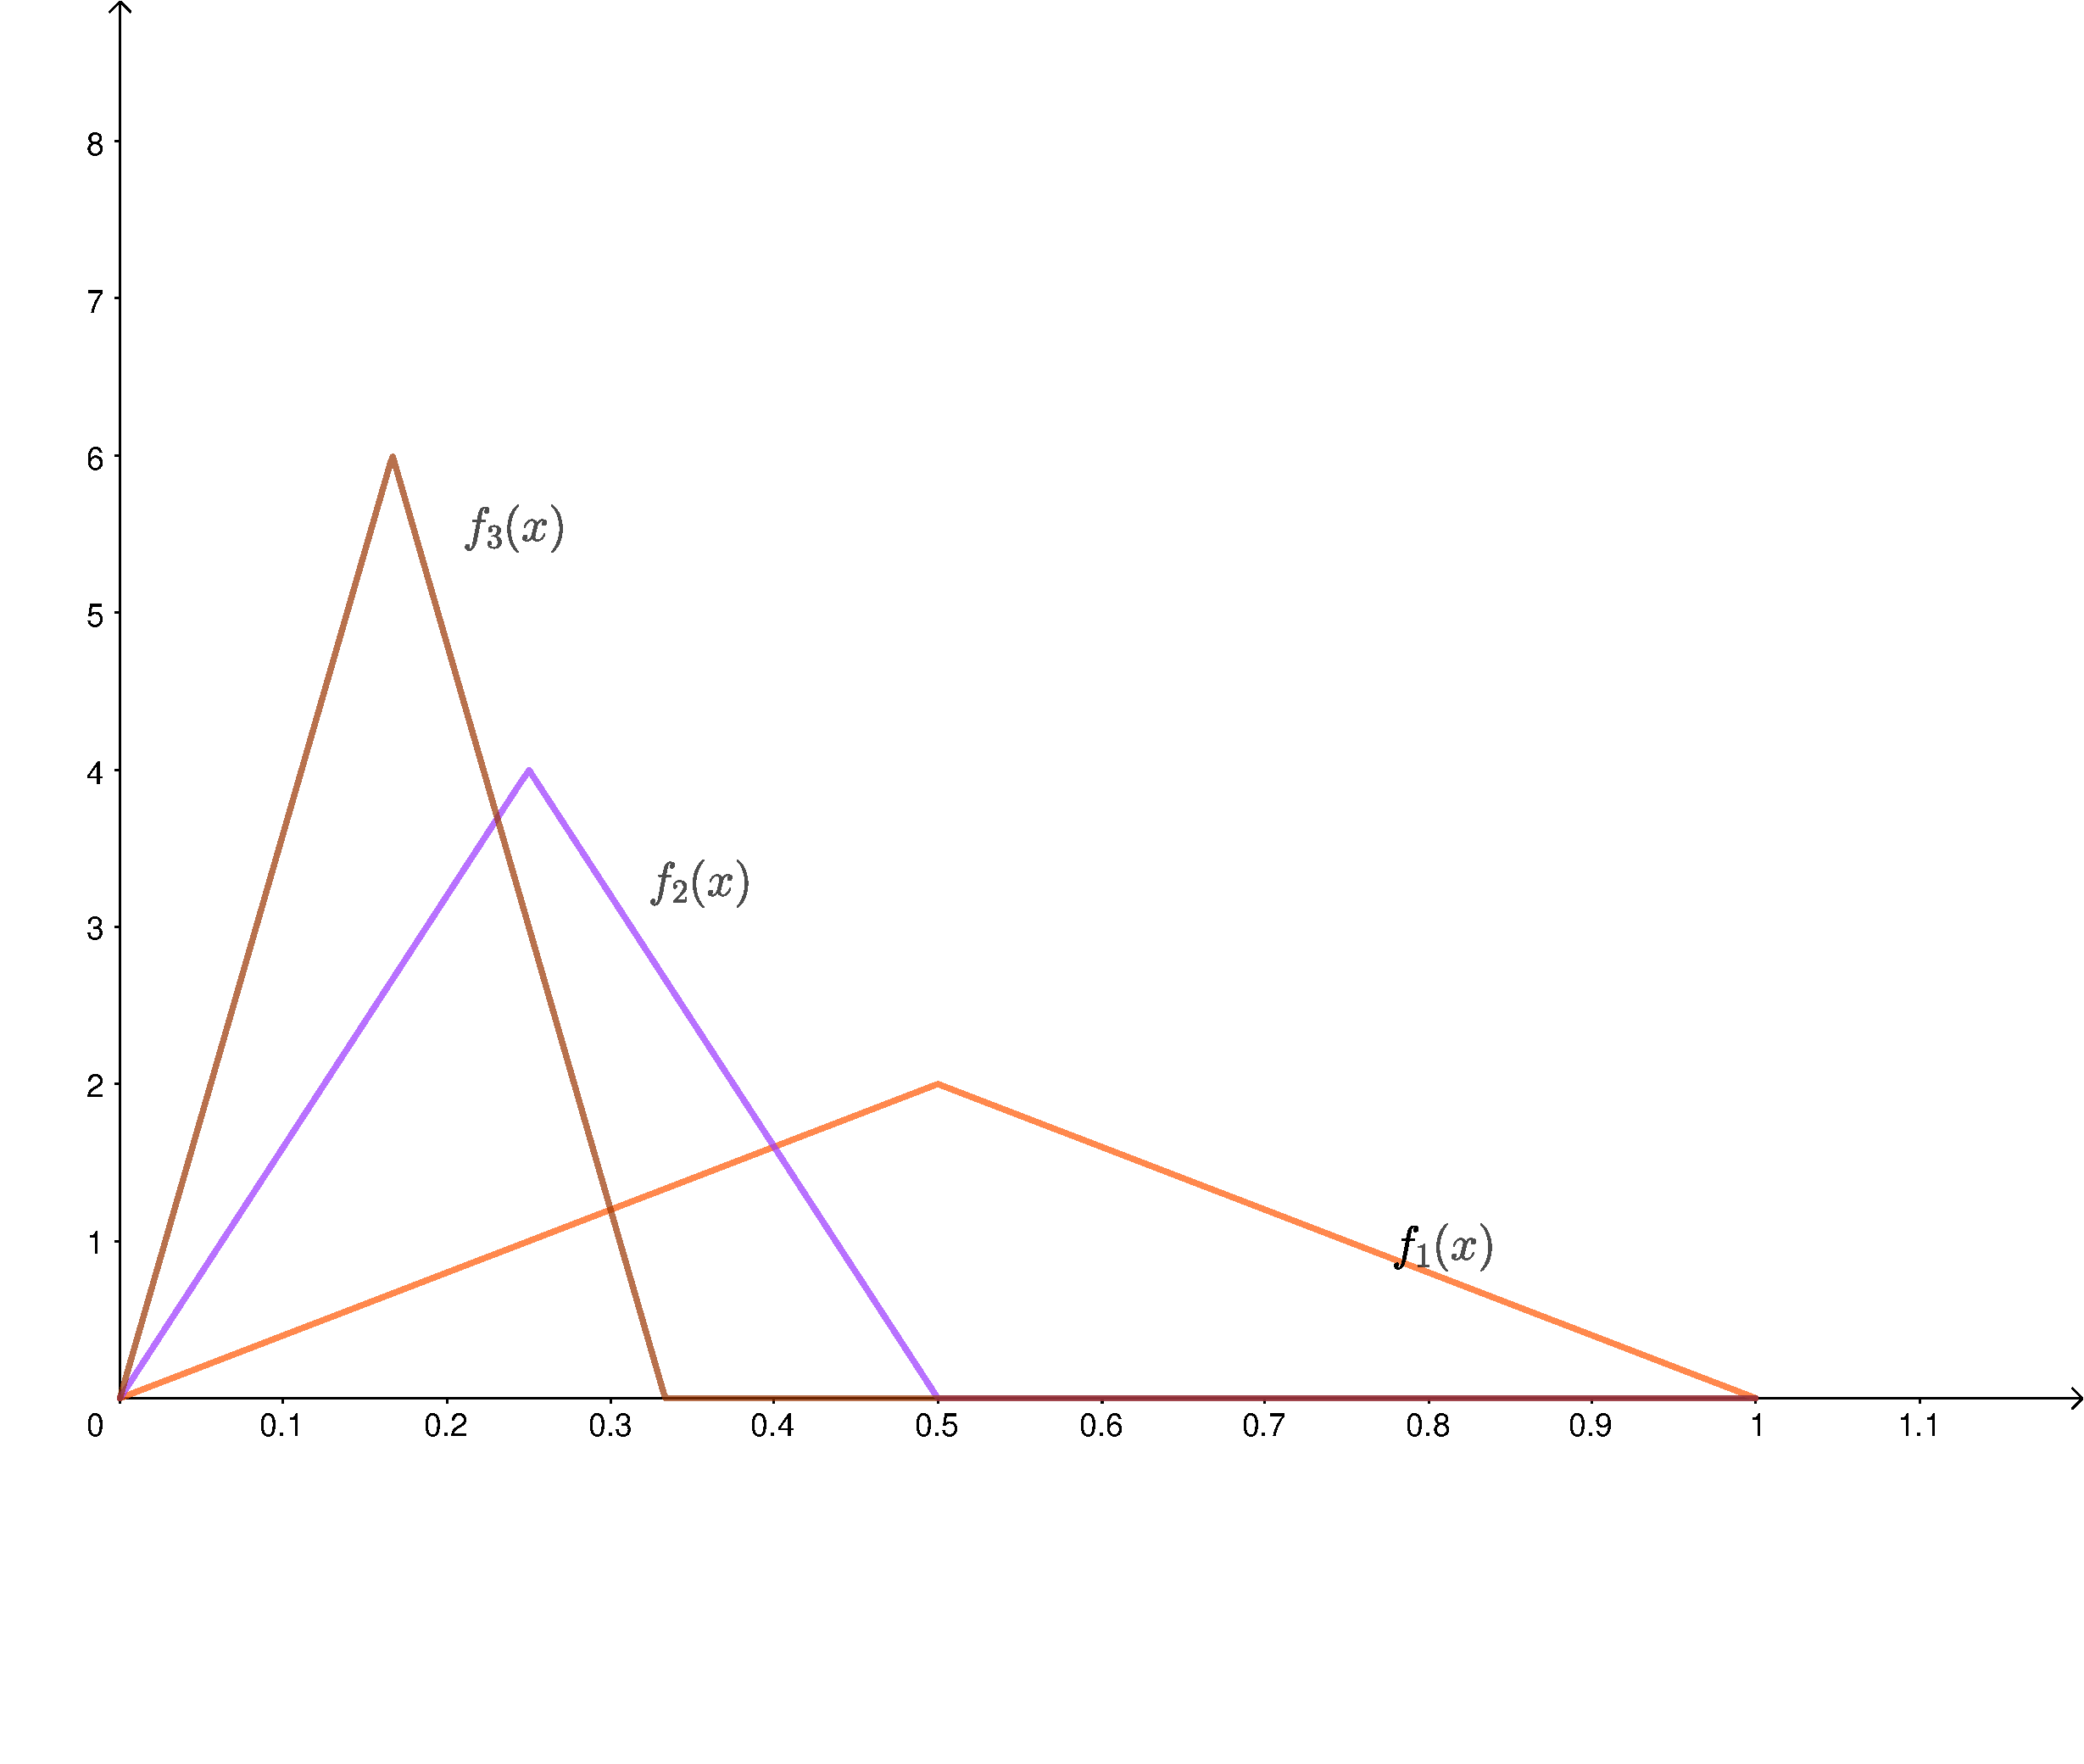
\includegraphics[width=0.75\textwidth]{images/06_sequence_functions.pdf}
    \centering
\end{figure}

\end{document}